% FPVR uses Meyer's Goals, Environment, System and Project requirements template.
% Legacy scientific-computing helper commands are retained for compatibility.
\documentclass[12pt]{article}
\usepackage{amsmath, mathtools}
\usepackage{amsfonts}
\usepackage{amssymb}
\usepackage{graphicx}
\usepackage{colortbl}
\usepackage{xr}
\usepackage{hyperref}
\usepackage{longtable}
\usepackage{xfrac}
\usepackage{tabularx}
\usepackage{float}
\usepackage{siunitx}
\usepackage{booktabs}
\usepackage{caption}
\usepackage{pdflscape}
\usepackage{afterpage}
\usepackage[numbers]{natbib}
\usepackage{graphicx}
\usepackage{float}
\setlength{\parindent}{0pt}
\setlength{\parskip}{0.75em}

%\usepackage{refcheck}
\hypersetup{
    bookmarks=true,         % show bookmarks bar?
      colorlinks=true,       % false: boxed links; true: colored links
    linkcolor=red,          % color of internal links (change box color with linkbordercolor)
    citecolor=green,        % color of links to bibliography
    filecolor=magenta,      % color of file links
    urlcolor=cyan           % color of external links
}
\input{../Comments.text}
\input{../Common.text}
% For easy change of table widths
\newcommand{\colZwidth}{1.0\textwidth}
\newcommand{\colAwidth}{0.13\textwidth}
\newcommand{\colBwidth}{0.82\textwidth}
\newcommand{\colCwidth}{0.1\textwidth}
\newcommand{\colDwidth}{0.05\textwidth}
\newcommand{\colEwidth}{0.8\textwidth}
\newcommand{\colFwidth}{0.17\textwidth}
\newcommand{\colGwidth}{0.5\textwidth}
\newcommand{\colHwidth}{0.28\textwidth}
% Used so that cross-references have a meaningful prefix
\newcounter{defnum} %Definition Number
\newcommand{\dthedefnum}{GD\thedefnum}
\newcommand{\dref}[1]{GD\ref{#1}}
\newcounter{datadefnum} %Datadefinition Number
\newcommand{\ddthedatadefnum}{DD\thedatadefnum}
\newcommand{\ddref}[1]{DD\ref{#1}}
\newcounter{theorynum} %Theory Number
\newcommand{\tthetheorynum}{TM\thetheorynum}
\newcommand{\tref}[1]{TM\ref{#1}}
\newcounter{tablenum} %Table Number
\newcommand{\tbthetablenum}{TB\thetablenum}
\newcommand{\tbref}[1]{TB\ref{#1}}
\newcounter{assumpnum} %Assumption Number
\newcommand{\atheassumpnum}{A\theassumpnum}
\newcommand{\aref}[1]{A\ref{#1}}
\newcounter{goalnum} %Goal Number
\newcommand{\gthegoalnum}{GS\thegoalnum}
\newcommand{\gsref}[1]{GS\ref{#1}}
\newcounter{instnum} %Instance Number
\newcommand{\itheinstnum}{IM\theinstnum}
\newcommand{\iref}[1]{IM\ref{#1}}
\newcounter{reqnum} %Requirement Number
\newcommand{\rthereqnum}{R\thereqnum}
\newcommand{\rref}[1]{R\ref{#1}}
\newcounter{nfrnum} %NFR Number
\newcommand{\rthenfrnum}{NFR\thenfrnum}
\newcommand{\nfrref}[1]{NFR\ref{#1}}
\newcounter{lcnum} %Likely change number
\newcommand{\lthelcnum}{LC\thelcnum}
\newcommand{\lcref}[1]{LC\ref{#1}}
\usepackage{fullpage}
\newcommand{\deftheory}[9][Not Applicable]
{
\newpage
\noindent \rule{\textwidth}{0.5mm}
\paragraph{RefName: } \textbf{#2} \phantomsection
\label{#2}
\paragraph{Label:} #3
\noindent \rule{\textwidth}{0.5mm}
\paragraph{Equation:}
#4
\paragraph{Description:}
#5
\paragraph{Notes:}
#6
\paragraph{Source:}
#7
\paragraph{Ref.\ By:}
#8
\paragraph{Preconditions for \hyperref[#2]{#2}:}
\label{#2_precond}
#9
\paragraph{Derivation for \hyperref[#2]{#2}:}
\label{#2_deriv}
#1
\noindent \rule{\textwidth}{0.5mm}
}
% Meyer template helpers required by the middle sections.
\usepackage{xcolor}
% Keep the supplied descriptions visible while drafting.
% Change to \showguidancefalse before submitting your completed SRS.
\newif\ifshowguidance
\showguidancefalse
\newcommand{\guidance}[1]{%
  \ifshowguidance
    \par\smallskip\begingroup\small\color{gray}
    \noindent\textbf{Provided description:} #1\par\endgroup\medskip
  \fi
}
\newcommand{\unumbered}[1]{%
  \phantomsection\section*{#1}\addcontentsline{toc}{section}{#1}}
\newcommand{\booksection}[2]{%
  \clearpage\unumbered{(#1) #2}
  \renewcommand{\thesubsection}{#1.\arabic{subsection}}
  \renewcommand{\theHsubsection}{#1.\arabic{subsection}}
  \setcounter{subsection}{0}}
\newcolumntype{Y}{>{\raggedright\arraybackslash}X}
\newcommand{\req}[1]{\hyperlink{req:#1}{\texttt{#1}}}
\newcommand{\ver}[1]{\hyperlink{ver:#1}{\texttt{#1}}}
\newcommand{\goal}[1]{\hyperlink{goal:#1}{#1}}
\newcommand{\haz}[1]{\href{../HazardAnalysis/HazardAnalysis.pdf\#haz:#1}{#1}}
\newcommand{\sym}[1]{\texttt{\detokenize{#1}}}
\newcommand{\proposal}{\textbf{PROPOSED; review pending.}}

\begin{document}

\title{Software Requirements Specification for \progname: Virtual Reality FPV Drone Training Simulator}

\author{\authname}

\date{October 19, 2026}

\maketitle

\clearpage

\pagenumbering{roman}

\tableofcontents

\clearpage

\section*{Revision History}

\begin{tabularx}{\textwidth}{@{}p{2.8cm}p{3.5cm}X@{}}
\toprule
\textbf{Date} & \textbf{Developer(s)} & \textbf{Changes} \\
\midrule

Oct 16, 2026 & Sankalpa &
Adapted the SRS document structure to Meyer's template. \\

\addlinespace

Oct 18, 2026 & Sankalpa &
Completed the Goals (G) section of the SRS. \\

\addlinespace
Oct 19, 2026 & AI-assisted draft &
Completed the Environment, System, and Project books and cross-document
traceability using the clarified scope; proposed specifications and validation
evidence remain subject to review. \\

\bottomrule
\end{tabularx}

\newpage

\clearpage

\clearpage

\listoftables

\listoffigures

\clearpage

\pagenumbering{arabic}

% The four books and numbered subsections 

% Write project content below each TODO. Guidance can be hidden globally.

\unumbered{Document conventions and baseline}\label{sec:conventions}
This software requirements specification (SRS) uses Meyer's Goals,
Environment, System, and Project books~\cite{BM22}. It is intended for the
development team, supervisor, evaluators, and prospective testers. Read the
Goals book for the intended value, the Environment book for the boundary and
terminology, and the System book for observable behaviour and acceptance.
The Project book records responsibilities, dependencies, and requirements
review work, rather than an approved whole-project calendar.

The current Goals book and the owner's October 19 clarifications
\cite{baseline} control intended scope. Earlier project documents remain
historical sources; this revision does not retroactively change them.
\textbf{Confirmed} denotes an owner-confirmed requirement in this specification,
not evidence of implementation. \textbf{PROPOSED} denotes a candidate that
requires team approval and is excluded from the confirmed acceptance baseline.
\textbf{TO BE REVIEWED} identifies an unresolved decision;
\textbf{PENDING VERIFICATION} identifies missing test or compatibility evidence.
No acceptance test, user interview, or safety validation is claimed here.

Requirement identifiers are stable: FR denotes functional requirements, NFR
non-functional requirements, SR proposed safety/security requirements, and
PR other proposed requirements. V identifies verification cases, HA hazards,
and LC/UC likely/unlikely changes. Quantities use the International System
of Units (SI): seconds, metres,
and their derived units); Hz is cycles per second and FPS is rendered frames
per second. The glossary in \hyperref[e1]{E.1} defines abbreviations and
formal symbols. A requirement's implementation is unconstrained unless an
external constraint is explicitly identified in \hyperref[e3]{E.3} or
\hyperref[p2]{P.2}.

To satisfy the rubric and checklists~\cite{rubric,srsChecklist,haChecklist},
this adaptation adds formal state rules in \hyperref[s2]{S.2}, a bidirectional
traceability register in \hyperref[s6]{S.6}, likely/unlikely changes in
\hyperref[p7]{P.7}, and a symbolic-constants appendix. These supplement the
Meyer headings without replacing them. Safety proposals link to the separate
\href{../HazardAnalysis/HazardAnalysis.pdf}{Hazard Analysis}.

\booksection{G}{Goals}

\subsection{Context and Overall Objectives}\label{g1}

Learning to operate a first-person-view (FPV) drone presents challenges for beginners, particularly when practicing with physical equipment. New pilots must develop coordinated flight-control skills while managing the possibility of crashes, equipment damage, and unsafe flight conditions. These challenges can make initial training costly and discourage inexperienced users from gaining practical experience.

FPVR is a virtual reality (VR)-based FPV drone training simulator designed to provide a safe, accessible, and structured environment for developing foundational drone piloting skills. The system will allow users to control a simulated drone, practice flight manoeuvres, and complete progressively challenging courses without requiring a physical drone.

The training environment will include free-flight practice, multiple obstacle-course levels, distinct virtual environments, checkpoints, and performance evaluation. Users will receive feedback on their flight performance through measurable indicators such as completion time, checkpoint progress, and performance ratings. An optional intelligent feedback component may provide further analysis of user performance.



\subsection{Current situation}\label{g2}

Learning to operate a first-person-view (FPV) drone requires beginners to develop coordinated control skills while interpreting visual feedback from the drone's perspective. Practicing with physical drones introduces risks of crashes, equipment damage, and additional costs, making simulation a valuable alternative for introductory training.

Several established FPV drone simulators, including Liftoff: FPV Drone Racing~\cite{liftoffFPV}  and VelociDrone\cite{velocidrone}, allow users to practice flight manoeuvres, complete racing courses, and explore virtual environments through conventional PC-based interfaces. These platforms provide extensive training and recreational capabilities, with a strong emphasis on realistic flight behaviour, racing, and freestyle flying. However, their traditional desktop experiences do not provide the same interaction environment as a dedicated virtual reality (VR) headset.

VR-based alternatives also exist. Liftoff: XR Drone~\cite{liftoffXR} introduces accessible drone flight using Meta Quest controllers, while DVR Simulator~\cite{dvrSimulator} and Drone Blitz~\cite{droneBlitz} offer VR flight challenges and racing or performance-tracking features. These applications demonstrate that immersive drone simulation is already feasible, but they differ in their emphasis on casual exploration, racing, and structured practice.

FPVR aims to build on these existing approaches by focusing specifically on a progressive, beginner-oriented VR training experience. Rather than treating flight practice and course completion as isolated activities, FPVR intends to connect free-flight familiarization, increasingly challenging obstacle courses, checkpoint-based objectives, and post-flight performance reviews into a continuous learning process. By allowing users to evaluate their results and repeat challenges, the system aims to help beginners recognize their mistakes and track improvements over successive attempts.

The intended contribution of FPVR is therefore not the introduction of drone simulation or VR flight itself, but the integration of immersive flight practice with structured progression and measurable feedback. The effectiveness of this approach will require evaluation with potential users.

\subsection{Expected Benefits}\label{g3}

\hypertarget{goal:G1}{}\textbf{Safe and Repeatable Practice (G1):}
FPVR will allow users to practice drone operation without exposing
a real drone or surrounding property to collision-related damage.
Users can recover from simulated crashes and repeat exercises
without the costs associated with damaging physical equipment.

\medskip

\hypertarget{goal:G2}{}\textbf{Progressive Skill Development (G2):}
Rather than relying exclusively on unrestricted flight, FPVR
will offer structured challenges of varying difficulty.
Users can freely select levels based on their experience and
practice increasingly demanding manoeuvres at their own pace.

\medskip

\hypertarget{goal:G3}{}\textbf{Performance Awareness (G3):}
After completing a training level, users will be able to
review their performance through recorded measures such as
completion time, checkpoint progress, and collisions.
This feedback is intended to help users identify areas for
improvement and encourage deliberate practice.

\medskip

\hypertarget{goal:G4}{}\textbf{Accessible Introductory Training (G4):}
FPVR will accommodate users with limited or no prior FPV
flying experience by providing a free-flight environment
where they can become familiar with flight controls before
attempting structured challenges.

\medskip

These benefits concern the intended training experience.
Any claim that FPVR improves actual physical-drone piloting
ability will require separate validation and is not assumed
by this specification.

\subsection{Functionality overview}\label{g4}

FPVR will provide the following capabilities to support
its goals.

\begin{table}[htbp]
\centering
\small
\caption{FPVR Functionality Overview}
\label{tab:functionality-overview}

\begin{tabularx}{\textwidth}{
    @{}p{4.0cm} X p{2.4cm}@{}
}
\toprule
\textbf{Functionality} &
\textbf{Description} &
\textbf{Initial Scope} \\
\midrule

VR Flight Experience &
First-person simulated drone flight through a virtual
reality headset. &
Core \\

\addlinespace

Free-Flight Practice &
An open-ended practice environment where users can
freely operate the drone without course objectives,
timers, or scoring. &
Core \\

\addlinespace

Obstacle-Course Levels &
Structured flight challenges of varying difficulty.
Users may select any available level regardless of
previous completion. &
Core \\

\addlinespace

Different Environments &
Multiple virtual environments for flight practice and
obstacle courses. Different levels may share the same
environment. &
Core \\

\addlinespace

Checkpoint System &
Designated course checkpoints used to track progress
toward level completion. &
Core \\

\addlinespace

Crash Recovery &
Following a simulated crash, users can choose to
restart the level or respawn at the most recently
reached checkpoint. &
Core \\

\addlinespace

Timing and Scoring &
Records completion time and calculates a score
based on defined performance measures during
obstacle-course challenges. &
Core \\

\addlinespace

Flight Review &
Provides a summary of flight performance after
completing a level, including completion time,
collisions, checkpoint results, and score. &
Core \\

\addlinespace

Flight Rating &
Provides a separate performance rating based on
defined flight measures. The evaluation criteria
remain to be determined. &
Core \\

\addlinespace

Intelligent Feedback &
Potential AI-based analysis of flight performance
to provide additional observations and recommendations,
subject to feasibility evaluation. &
Planned \\

\addlinespace

Controller Input &
Supports drone control using Meta Quest controllers
or a compatible Xbox controller. &
Core \\

\bottomrule
\end{tabularx}
\end{table}

The exact scoring and rating criteria, controller mappings,
checkpoint and respawn behaviour, and requirements for
AI-based feedback will be specified in the System section.


\subsection{High-level usage scenarios}\label{g5}

This section describes the primary interactions between
users and FPVR during flight practice, obstacle-course
completion, crash recovery, and performance evaluation.
These scenarios illustrate the intended system behaviour
and support the goals defined in Section G.1.

\subsubsection{Scenario 1: Initial Free-Flight Practice}

A first-time user launches FPVR and selects the free-flight
mode using either Meta Quest controllers or a compatible
Xbox controller. The user enters a virtual environment
where they can practice basic flight manoeuvres, such as
ascending, descending, turning, and navigating through
the environment.

Unlike structured obstacle-course levels, free-flight
mode has no checkpoints, timers, or scoring. Users can
explore and practice at their own pace without specific
completion objectives.

If the drone experiences a simulated crash, the user can
reset its position and continue practicing. The user may
leave free-flight mode and return to the level-selection
interface when desired.

This scenario supports G1 and G4 by providing a safe,
repeatable environment for becoming familiar with FPV
drone controls.


\subsubsection{Scenario 2: Completing an Obstacle-Course Level}

A user selects an obstacle-course level from the available
challenges. All levels are accessible regardless of previous
completion, allowing users to choose courses appropriate
to their experience and preferences.

Each level contains obstacles and a sequence of checkpoints
that must be completed in the designated order. The system
tracks the user's progression, total elapsed time, and time
spent navigating between checkpoints. Upon reaching a
checkpoint, the current section timer resets while the
total elapsed time continues accumulating.

The user navigates through the checkpoints in sequence
until reaching the finish. After successful completion,
the system calculates a numerical score and a separate
performance rating based on the recorded flight results.

The user can then review their performance, retry the
level, or select another challenge.

This scenario supports G2 by providing structured flight
challenges of varying difficulty with measurable outcomes.


\subsubsection{Scenario 3: Recovering from a Simulated Crash}

While attempting an obstacle-course level, the user loses
control of the drone and experiences a simulated crash.
The system records the collision and provides two recovery
options: restart the entire level or respawn at the most
recently reached checkpoint.

If the user selects respawn, the drone returns to the last
successfully reached checkpoint. If no checkpoints have
been reached, the drone returns to the level's starting
position.

The current section timer resets upon respawning, allowing
the user to attempt the section again. However, the total
elapsed time continues accumulating, including the time
spent on failed attempts. The recorded collision also
negatively affects the final score.

The user can continue attempting the course without
restarting the FPVR application.

This scenario supports G1 and G2 by allowing users to
recover from mistakes while maintaining meaningful
performance consequences.

\subsubsection{Scenario 4: Reviewing Flight Performance}

After successfully completing an obstacle-course level,
the user receives a flight review summarizing their
performance.

The review includes the total completion time, checkpoint
results, collision count, and numerical score. The total
completion time includes time spent on failed sections
and subsequent attempts following checkpoint respawns.

The system also presents a separate overall performance
rating based on defined evaluation criteria. The user can
examine these results to identify areas for improvement
before attempting another flight challenge.

This scenario supports G3 by providing measurable feedback
intended to encourage deliberate practice and improvement.

The exact scoring formula, rating categories, and penalties
associated with collisions must be established in \hyperref[s2]{S.2}.


\subsubsection{Scenario 5: AI-Assisted Flight Feedback
(Planned: Subject to Feasibility)}

If AI-assisted feedback is included in the final
implementation, the system will automatically provide
additional performance analysis as part of the post-level
flight review.

Using available flight-performance data, the system would
identify areas of difficulty and provide understandable
observations or recommendations. For example, the
feedback might highlight repeated collisions or
difficulties navigating particular obstacle sections.

The intelligent feedback component is intended to
complement the standard numerical score and performance
rating rather than replace them.

The feasibility, data requirements, analysis approach,
and evaluation criteria for AI-assisted feedback remain
to be determined. The standard flight review will remain
available independently of this optional capability.

\begin{figure}[H]
    \centering
    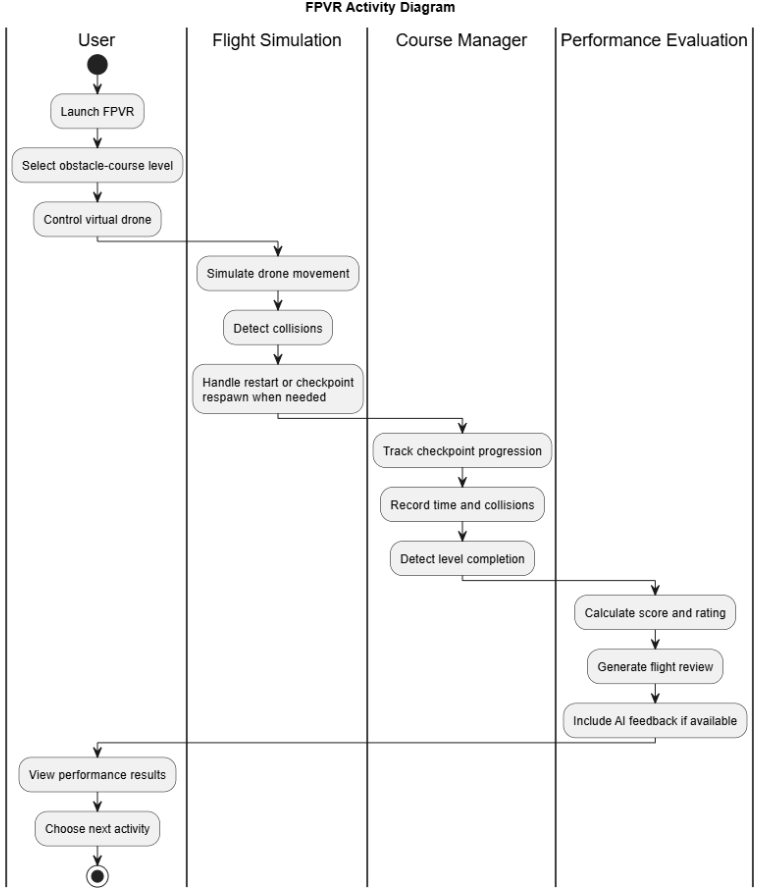
\includegraphics[width=0.85\textwidth]{activityDiagram.png}
    \caption{High-Level FPVR Training Activity Diagram}
    \label{fig:high-level-activity}
\end{figure}
The activity diagram illustrates the primary
obstacle-course training workflow. Swimlanes
identify the responsible user or system
component, while arrows indicate the sequence
of activities.
\subsection{Limitations and Exclusions}\label{g6}

FPVR is intended to provide an introductory virtual reality
(VR) training experience for first-person-view (FPV) drone
operation. The following limitations and exclusions define
the boundaries of the system and clarify functionality
outside the project's current scope.

\newpage
\begin{table}[htbp]
\centering
\small
\caption{FPVR Limitations and Exclusions}
\label{tab:limitations-exclusions}

\begin{tabularx}{\textwidth}{
    @{}p{4cm} X@{}
}
\toprule
\textbf{Area} &
\textbf{Limitation or Exclusion} \\
\midrule

Physical Drone Operation &
FPVR is limited to simulated drone operation and will not
communicate with or control physical drones. \\

\addlinespace

VR Hardware Requirement &
FPVR requires a compatible VR headset for operation.
Both Meta Quest controllers and compatible Xbox controllers
will be supported, but conventional PC gameplay without
a VR headset is excluded. \\

\addlinespace

Pilot Certification &
FPVR will not provide official drone pilot certification
or replace applicable regulatory examinations, assessments,
or licensing requirements. \\

\addlinespace

Real-World Flight Proficiency &
Performance within FPVR will not be considered proof
of a user's ability to safely operate a physical drone.
The transfer of skills from simulation to real-world
flight is not guaranteed. \\

\addlinespace

Flight Simulation Realism &
FPVR aims to provide realistic flight behaviour for
training purposes. However, the underlying flight model,
its implementation, and the required level of accuracy
remain under review. The system is not intended to
reproduce every physical and environmental characteristic
of real-world drone operation. \\

\addlinespace

Multiplayer Functionality &
FPVR is limited to single-player training.
Multiplayer racing, cooperative flight, and shared
online training sessions are excluded. \\

\addlinespace

Dedicated FPV Transmitters &
Support for dedicated FPV radio transmitters is under
consideration but is not part of the confirmed core
controller requirements. Compatibility and feasibility
will be evaluated during development. \\

\addlinespace

Historical Flight Records &
FPVR will provide performance reviews after completing
obstacle-course levels but will not include functionality
for accessing or reviewing previously completed sessions. \\

\addlinespace

AI-Assisted Feedback &
AI-generated flight feedback is planned subject to
feasibility evaluation. Core flight reviews, numerical
scores, and performance ratings will remain available
independently of this optional capability. \\

\bottomrule
\end{tabularx}
\end{table}

FPVR focuses on safe introductory flight practice,
structured obstacle-course challenges, and performance
evaluation within a virtual environment. The system
is not intended to replace real-world flight training
or serve as a comprehensive engineering-grade flight
simulator. The risks associated with these limitations and their corresponding
mitigation strategies are discussed in
\hyperref[p6]{P.6}.


\subsection{Stakeholders and requirements sources}\label{g7}

This section identifies the stakeholders who may influence
or be affected by FPVR and the sources used to establish
its initial requirements. It distinguishes confirmed
project participants from potential stakeholders whose
feedback has not yet been collected.

\subsubsection{Stakeholders}

Table~\ref{tab:stakeholders} identifies the primary
and secondary stakeholders of FPVR and their interests
in the project.

\begin{table}[htbp]
\centering
\small
\caption{FPVR Stakeholders}
\label{tab:stakeholders}

\begin{tabularx}{\textwidth}{@{}p{3.4cm} X@{}}
\toprule
\textbf{Stakeholder} &
\textbf{Interest in FPVR} \\
\midrule

Beginner FPV Pilots &
Primary intended users seeking accessible introductory
training, opportunities to practise basic flight
manoeuvres, and feedback on their performance. \\

\addlinespace

Drone Enthusiasts &
Potential users interested in additional flight practice,
structured challenges, and evaluating the realism of
the simulation. \\

\addlinespace

Students and Technology Enthusiasts &
Potential users interested in experiencing FPV drone
operation through virtual reality. Intended use is
subject to applicable headset age and safety
restrictions. \\

\addlinespace

McMaster Drone Team &
Potential technical stakeholder that may provide
feedback on simulated drone behaviour
and operator training. The team has not yet been
consulted. \\

\addlinespace

Project Team &
Responsible for developing, testing, maintaining,
and documenting FPVR according to the established
requirements. \\

\addlinespace

Project Supervisor &
Provides technical guidance and feedback on project
scope, feasibility, and simulation realism. \\

\addlinespace

Course Evaluators &
Review the project's requirements, engineering
process, documentation, and delivered functionality
against the course expectations. \\

\addlinespace

Parents and Guardians &
Indirect stakeholders concerned with age-appropriate
access and the safe use of VR by younger users. \\

\addlinespace

Society and General Public &
Indirect stakeholders interested in safer introductory
drone training, responsible technology use,
accessibility, and the management of VR-related
health and safety concerns. \\

\bottomrule
\end{tabularx}
\end{table}

Society is considered an indirect stakeholder because
VR-based drone training has implications for physical
safety, user well-being, accessibility, and responsible
drone operation. FPVR must not misrepresent simulated
flight performance as proof of real-world piloting
competence.

FPVR is intended for users with varying levels of
experience and age, subject to the age restrictions
and safety requirements of the supported VR hardware.
Applicable platform age-group requirements are
documented by Meta~\cite{metaAgeGroups}.


\subsubsection{Requirements Sources}

The initial requirements for FPVR have been developed
using existing project documentation, team discussions,
supervisor guidance, and technical references relevant
to virtual reality and flight simulation.

The principal requirements sources are summarized
in Table~\ref{tab:requirements-sources}.

\begin{table}[htbp]
\centering
\small
\caption{FPVR Requirements Sources}
\label{tab:requirements-sources}

\begin{tabularx}{\textwidth}{@{}p{3.5cm} X@{}}
\toprule
\textbf{Source} &
\textbf{Contribution to Requirements} \\
\midrule

Problem Statement &
Establishes the problem being addressed, the
project's objectives, and its intended benefits. \\

\addlinespace

Development Plan &
Provides project scope, planned development
activities, technical considerations, and
project constraints. \\

\addlinespace

Hazard Analysis &
Identifies potential hazards and safety
considerations relevant to the simulator
and its users. \\

\addlinespace

Supervisor Discussions and Meeting Notes &
Provide technical guidance on simulation realism,
drone flight behaviour, and the selection of
an appropriate flight model. \\

\addlinespace

Unity Documentation &
Provides information about available physics
simulation capabilities, including movement,
forces, gravity, and collision handling
\cite{unityRigidbody}. \\

\addlinespace

Meta Quest Documentation &
Provides technical information about VR device
integration and controller input
\cite{metaQuestInput}, as well as applicable
age-group requirements \cite{metaAgeGroups}. \\

\addlinespace

Existing FPV Simulators &
Provide a basis for comparing existing flight
practice, training, and performance evaluation
capabilities with the proposed functionality
of FPVR. \\

\addlinespace

Potential End Users &
Planned source of feedback on usability,
flight-control expectations, training needs,
and the effectiveness of performance feedback.
Direct consultation has not yet occurred. \\

\bottomrule
\end{tabularx}
\end{table}

The project supervisor has provided guidance
concerning realistic flight behaviour and the
selection of an existing drone model as a possible
basis for the simulation. These discussions have
informed the identification of technical concerns,
but the final flight model and required accuracy
remain under review.

No structured requirements-elicitation sessions
have yet been conducted with the intended end users.
The project team plans to consult potential users,
including beginners and individuals familiar with
drone operation, to validate assumptions about
usability, training needs, and performance feedback.

Until this consultation takes place, the identified
user needs and evaluation targets remain provisional.
Feedback collected during development will be used
to review and refine the system requirements.

\subsection{User Profiles}\label{g8}

FPVR is intended for users with varying levels of
experience in drone operation, virtual reality (VR),
and video games. The system primarily targets
beginners while also accommodating recreational
users and experienced FPV pilots. Users must comply
with the age and safety restrictions of the
supported VR hardware.

The following profiles describe the anticipated
experience, needs, and usage patterns of the
system's main user groups.


\subsubsection{Novice FPV Pilot}
\label{sec:novice-user}

The primary user is an individual with little or
no experience operating first-person-view (FPV)
drones. This user may also be unfamiliar with
VR environments and their associated controllers.

\noindent\textbf{Experience:}
May have general familiarity with computers or
video games but limited knowledge of drone flight
controls, navigation, and flight behaviour.

\noindent\textbf{Needs:}
Clear control instructions, understandable
interactions, opportunities to practise without
risking damage to physical equipment, and
feedback on flight performance.

\noindent\textbf{Expected Usage:}
The user reviews the basic control instructions
and begins practising in free-flight mode.
As confidence improves, the user may select
obstacle-course levels of increasing difficulty.
Progression is voluntary, as all levels are
available without prerequisite completion.


\subsubsection{Casual Gamer or Technology Enthusiast}
\label{sec:casual-user}

This user is interested in experiencing drone
flight through VR without necessarily intending
to purchase or operate a physical drone.

\noindent\textbf{Experience:}
May be familiar with video-game controllers and
immersive experiences but have limited knowledge
of actual FPV drone operation.

\noindent\textbf{Needs:}
Engaging virtual environments, accessible
controls, understandable objectives, and
opportunities to measure improvement through
repeated challenges.

\noindent\textbf{Expected Usage:}
The user explores free-flight environments
and attempts obstacle-course challenges for
recreation and exploration. The user may
repeat levels to improve completion times,
scores, and performance ratings.


\subsubsection{Experienced FPV Pilot or Technical Evaluator}
\label{sec:experienced-user}

This user has prior experience operating physical
FPV drones or working with related technical
systems. Experienced users may participate in
regular training activities or provide feedback
during system evaluation.

\noindent\textbf{Experience:}
Familiar with drone controls, flight manoeuvres,
and the expected behaviour of physical drones.

\noindent\textbf{Needs:}
Consistent control responses, meaningful
obstacle-course challenges, and sufficient
performance information to evaluate the
simulator's behaviour.

\noindent\textbf{Expected Usage:}
The user practises in free-flight mode,
completes obstacle-course challenges, and
reviews recorded performance results.
The user may also compare simulated flight
behaviour with prior experience and identify
areas for improvement. The required accuracy
of the underlying flight model remains
under review.


\subsubsection{General User Considerations}
\label{sec:general-user-considerations}

FPVR is intended to accommodate both seated and
standing operation using a compatible VR headset.
Users may interact with the simulator through
Meta Quest controllers or compatible Xbox
controllers.

Users may differ in physical capabilities,
experience with immersive environments, and
susceptibility to VR-related discomfort.
The system's design will consider applicable
headset safety guidance and the needs of
different user groups.

The profiles presented in this section are
based on the intended target audience rather
than completed user interviews. As discussed
in Section~\ref{g7},
the project team plans to consult potential
users to validate their needs, expectations,
and usage assumptions.



\booksection{E}{Environment}

\guidance{The Environment book describes the application domain and external context, physical or virtual (or a mix), in which the system will operate. \cite{BM22}}

\subsection{Glossary}\label{e1}

\guidance{Clear and precise definitions of all the vocabulary specific to the application domain, including technical terms, words from ordinary language used in a special meaning, and acronyms. It introduces the terminology of the project; not just of the environment in the strict sense, but of all its parts. \cite{BM22}}

\begin{longtable}{@{}p{0.23\textwidth}p{0.72\textwidth}@{}}
\caption{Glossary and abbreviations}\label{tab:glossary}\\
\toprule Term & Definition \\ \midrule\endfirsthead
\toprule Term & Definition \\ \midrule\endhead
\bottomrule\endfoot
FPV & First-person view: the simulated drone's viewing perspective; introduced
in \hyperref[g1]{G.1}. \\
VR & Virtual reality: headset-mediated immersive presentation; introduced in
\hyperref[g1]{G.1}. \\
SRS & Software requirements specification; defined in the
\hyperref[sec:conventions]{reading guide}. \\
AI & Artificial intelligence; the optional intelligent-feedback capability in
\hyperref[sec:s2-ai]{S.2}. Existing Goals references to AI refer to this capability. \\
PC / PCVR & Personal computer / computer-executed virtual reality, displayed
through the headset; see \hyperref[e2]{E.2}. \\
XR / OpenXR & Extended reality / the Khronos runtime interface for XR
applications; the imposed Unity choice does not mandate a particular XR package
version (\hyperref[p2]{P.2}). \\
FPS / Hz & Frames per second / hertz; application frame delivery and display
refresh are distinct quantities (\hyperref[sec:proposed-performance]{S.2}). \\
V\&V / QA & Verification and validation / quality assurance;
\hyperref[s6]{S.6} and \hyperref[p1]{P.1}. \\
FMEA / HA & Failure mode and effect analysis / Hazard Analysis;
see \href{../HazardAnalysis/HazardAnalysis.pdf}{the companion document}. \\
API & Application programming interface, an interface between programs;
\hyperref[s3]{S.3} does not commit to a public API. \\
VRC & Virtual reality check, Meta's distribution acceptance criteria;
see \hyperref[e3]{E.3}. \\
ML / RF & Machine learning / radio frequency; optional investigation terminology
in \hyperref[p1]{P.1} and \hyperref[p2]{P.2}, not core feature commitments. \\
SI & International System of Units; see the
\hyperref[sec:conventions]{reading guide}. \\
Attempt & One obstacle-course run from start/restart through completion or exit;
respawn continues that attempt. \\
Checkpoint / segment & An ordered course gate / flight between successive gates
or between a start/gate and the finish. \\
Crash & A single latched simulated collision event; it cannot repeat while the
same crash awaits recovery. \\
Respawn / restart & Resume the same attempt at its last completed checkpoint /
create a new attempt from the level start. \\
Score / rating & A numerical result / a separate category describing the current
attempt; neither certifies real-world skill. \\
Tracking / focus & Runtime-reported pose information / permission to receive XR
interaction; visible imagery does not imply valid, active input. \\
Native frame & A new application-rendered frame, excluding synthetic or repeated
frames supplied by the runtime. \\
Telemetry & Current-attempt flight/performance measurements; external transfer
and persistent history are not confirmed features. \\
\end{longtable}

\begin{table}[htbp]\centering\small
\caption{Symbols used in the formal requirements}\label{tab:symbols}
\begin{tabularx}{\textwidth}{@{}p{0.22\textwidth}Y@{}}\toprule
Symbol & Meaning and unit \\ \midrule
$n,k,C_i$ & Number of required checkpoints / completed prefix length (integers)
/ the checkpoint with sequence index $i$, where $1\leq i\leq n$. \\
$q,q_{\rm saved},a$ & Session state / saved state before a proposed interruption /
airborne flag (Boolean for $a$). \\
$T,U,c$ & Accumulated active-flight time, current-segment time (s), crash count. \\
$\Delta t,t$ & Non-negative elapsed interval between observations / elapsed
gravity-fixture time (s). A prime denotes a value after a transition. \\
$p_k$ & Recovery pose for completed prefix $k$; $p_0$ is the start pose. \\
$T_r,B,P,S$ & Positive course reference time (s), score base, crash penalty,
and resulting numerical score (dimensionless points). \\
$R,\rho,\gamma$ & Rating category, permitted time ratio, and rating crash limit. \\
$f_{\min},b_f,L_{\max}$ & Proposed native frame target (FPS), frame budget (ms),
and application-receipt-to-visible-response latency limit (ms). \\
$h_{\rm TO},g,\epsilon$ & Proposed takeoff clearance (m), reference gravity
(m/s$^2$), and relative gravity-check tolerance. \\
$x,y,\theta$ & Horizontal/vertical stick axes and normalized throttle command. \\
$\land,\lor,\Rightarrow$ & Logical and, or, and implication. \\
$\mathbb N_0,\mathbb R_{\geq0}$ & Non-negative integers and non-negative reals. \\
\bottomrule\end{tabularx}\end{table}

Numerical values and approval status are defined once in
Appendix~\ref{app:constants}; references elsewhere use their symbolic names.
In diagrams, a rectangle identifies an actor, external dependency, or logical
FPVR responsibility as labelled. A labelled arrow denotes information flow,
not a physical wire or an implementation module dependency.

\subsection{Components}\label{e2}

\guidance{List of elements of the environment that may affect or be affected by the system and project. It includes other systems to which the system must be interfaced. These components may include existing systems, particularly software systems, with which the system will interact --- by using their APIs (program interfaces), or by providing APIs to them, or both. These are interfaces provided to the system from the outside world. They are distinct from both: interfaces provided by the system to the outside world (\hyperref[s3]{S.3}); and technology elements that the system's development will require (\hyperref[p5]{P.5}). \cite{BM22}}

The external environment contains the user and their physical activity space;
the Quest headset, motion controllers, and runtime; an Xbox-compatible
controller where supported; and, for PCVR, the host computer and headset link.
The standalone device executes FPVR locally; PCVR executes it on the host and
uses the headset for presentation. These are separate deployment paths, not
simultaneous execution requirements. No physical drone belongs to either path.

\begin{table}[htbp]\centering\small
\caption{External components and boundary interactions}\label{tab:external}
\begin{tabularx}{\textwidth}{@{}p{0.24\textwidth}YY@{}}\toprule
External component & Inputs to FPVR & Outputs from FPVR \\ \midrule
User & Mode/level choice, flight axes, menu actions, recovery choice &
Flight view, instructions, checkpoint state, recovery options, current results \\
Quest/runtime & Pose validity, input availability, session focus, display timing &
Rendered imagery and application lifecycle responses \\
Quest or Xbox input device & Controller identity, bounded axes/buttons,
connection state & Displayed mapping and connection feedback \\
PCVR host/link & Runtime/device availability, controller events, host resources &
PC-executed session displayed through the headset \\
Physical space/guardian & Safe-use preparation outside software control &
Proposed safety reminders; FPVR cannot guarantee a clear physical space \\
Optional AI service & Optional analysis result or failure & No core output;
proposed opt-in minimum data only if external analysis is approved \\
\bottomrule\end{tabularx}\end{table}

\begin{figure}[htbp]\centering\small
\fbox{\begin{minipage}{0.94\textwidth}\centering
User and physical surroundings\\[3pt]
$\xrightarrow{\text{choices, controls}}$
\fbox{FPVR: flight, course state, evaluation, VR interfaces}
$\xrightarrow{\text{imagery, instructions, results}}$ User\\[6pt]
Quest runtime / controllers / PCVR host
$\xrightarrow{\text{pose, input, focus, timing}}$ FPVR\\[3pt]
FPVR $\xrightarrow{\text{frames, lifecycle response}}$ Quest runtime\\[6pt]
FPVR $\xrightarrow{\text{optional, separately approved data}}$
AI dependency $\xrightarrow{\text{feedback or failure}}$ FPVR
\end{minipage}}
\caption{FPVR context and information-flow boundary. The AI connection is
conditional; arrows identify data direction, not an approved network design.}
\label{fig:context}\end{figure}

\subsection{Constraints}\label{e3}

\guidance{Obligations and limits imposed on the project and system by the environment. This chapter defines non-negotiable restrictions coming from the environment (business rules, physical laws, engineering decisions), which the development will have to take into account. \cite{BM22}}

\begin{description}
\item[C-01: Deployment.] Unity development, a required VR headset, both
standalone Quest and PCVR execution, and the two overall controller types are
owner-imposed constraints~\cite{baseline}. They preserve the intended immersive
training experience and support flexible hardware access; they do not establish
that every hardware/controller combination works.
\item[C-02: Primary hardware.] Meta Quest 3S is the intended primary headset.
Equivalent/additional Quest models, Xbox generations, PC operating systems,
minimum host specifications, and the per-mode controller matrix are
\textbf{TO BE REVIEWED}. Windows is a candidate PCVR target, not an approved
platform guarantee. \ver{V-08} must record the exact tested configuration.
\item[C-03: External safety and platform obligations.] Use must follow the
applicable model/region's Meta age eligibility, supervision, and safety
instructions~\cite{metaSafety,metaAgePolicy}. A broad audience does not imply
unrestricted child suitability. Distribution, parental controls, applicable
privacy obligations, and accessibility obligations require a release review;
no jurisdiction-specific compliance or legal certification is asserted here.
\item[C-04: Distribution checks.] Meta's VRC guidance and runtime lifecycle
rules inform testing~\cite{metaVRC,metaLifecycle,openXR}. They are external
distribution conditions if a Meta release is pursued, not proof that FPVR
passes them. The proposed native-frame target is an engineering choice, not
a claim that Meta universally mandates that rate.
\item[C-05: Scope.] Exclusions in \hyperref[g6]{G.6} are binding. Multiplayer,
desktop-only play, physical-drone control, certification, and historical review
are absent from the baseline. The Development Plan's earlier wider possibilities
are historical context, not additional requirements.
\end{description}

\subsection{Assumptions}\label{e4}

\guidance{Properties of the environment that may be assumed, with the goal of facilitating the project and simplifying the system. It defines properties that are not imposed by the environment (like those in \hyperref[e3]{E.3}) but assumed to hold, as an explicit decision meant to facilitate the system's construction. \cite{BM22}}

These explicit operating premises describe the intended environment. Their
failure is analysed in the Hazard Analysis rather than assumed impossible.
\begin{description}
\item[A-01: Runtime availability.] A selected configuration can launch a
compatible XR runtime and report session/input status. This is needed to attempt
VR operation; successful compatibility remains \textbf{PENDING VERIFICATION}
under \ver{V-08}. Link failure, focus loss, and stale pose remain hazards
\haz{HA-04}, \haz{HA-14}, and \haz{HA-16}.
\item[A-02: Activity-space preparation.] Users or guardians can consult the
headset instructions and prepare a suitable stationary space. This does not
assume that users always comply or that the platform boundary prevents impacts;
\haz{HA-01}/\haz{HA-03} and proposed \req{SR-01} address those limitations.
\item[A-03: Course configuration.] Each released course supplies a start pose,
ordered checkpoints, finish, collision surfaces, and safe recovery poses.
Validation is required; corrupt or impossible configurations remain
\haz{HA-08} and motivate proposed \req{SR-05}.
\item[A-04: Evaluation access.] Tests can access a selected headset/controller
combination and representative courses. Their availability is a project
dependency, not evidence that any test has run. Missing equipment blocks that
configuration's acceptance rather than implying compatibility.
\end{description}
External AI access, uninterrupted tracking, perfect user health, and crash-free
software are deliberately not assumptions. The core's proposed offline behaviour
and optional-AI failure fallback are separately specified requirements.

\subsection{Effects}\label{e5}

\guidance{Elements and properties of the environment that the system will affect. It defines effects of the system's operations on properties of the environment. Where the previous two categories (\hyperref[e3]{E.3}, \hyperref[e4]{E.4}) defined influences of the environment on the system, effects are influences in the reverse direction. \cite{BM22}}

FPVR changes only simulated state, displayed imagery, and the current attempt's
performance record. It gives users repeatable practice without commanding a
physical drone. Its imagery may still cause discomfort, distract from nearby
objects, or create unjustified confidence about real-world skill. These effects
are analysed in \haz{HA-01}, \haz{HA-02}, \haz{HA-06}, and \haz{HA-17}.

The current-attempt dataset comprises the chosen level, checkpoint prefix,
active timers, crash count, score, rating, and any optional feedback inputs.
No account, telemetry export, external transmission, or persistent-history
feature is confirmed. Proposed \req{SR-06}--\req{SR-08} constrain those effects
if approved. Human safety/accessibility evaluation remains
\textbf{PENDING VERIFICATION}; in-simulator success is not a safety assurance.

\subsection{Invariants}\label{e6}

\guidance{Properties of the environment that the system's operation must preserve, i.e., properties of the environment that operations of the system may assume to hold when they start, and must maintain. \cite{BM22}}

\begin{description}
\item[I-01: Physical boundary.] No session action produces a physical-drone
command, and no score or rating represents pilot certification (\hyperref[g6]{G.6}).
\item[I-02: Course integrity.] A completed checkpoint prefix remains ordered;
respawn preserves it, while restart replaces the attempt. The precise invariant
and transitions are in \hyperref[sec:formal]{S.2}.
\item[I-03: Stationary interaction.] Both seated and standing use remain
possible without walking to steer, operate menus, or recover
(\req{FR-UI-06}, \req{NFR-SAFE-01}).
\item[I-04: Independent core review.] Optional intelligent feedback never
becomes a prerequisite for the standard review (\req{FR-REV-04},
\req{FR-AI-03}); proposed \req{SR-08} additionally prevents AI from rewriting
the authoritative result.
\end{description}
An invariant is a required property, not an assertion that an unfinished
implementation already preserves it. Exceptional exits and lost runtime access
are subject to \hyperref[s4]{S.4} and \ver{V-12}.

\booksection{S}{System}

\guidance{The System book refines the Goals one by focusing on more detailed requirements. It describes the system itself: its components, its functionality, and the criteria by which an implementation will be judged satisfactory. \cite{BM22}}


\subsection{Components}\label{s1}

\guidance{Overall structure expressed by the list of major software and, if applicable, hardware parts. \cite{BM22}}

The following are logical responsibilities for specifying behaviour, not a
module design: (1) drone flight and collision; (2) training modes and level
selection; (3) checkpoint progression and recovery; (4) timing and evaluation;
(5) VR interfaces and controller input; (6) post-flight review; and (7) optional
intelligent feedback. Each has a corresponding subsection of \hyperref[s2]{S.2}.
The first six comprise the core. The seventh is conditional on a separate
feasibility and scope decision. Safety, validation, and deployment properties
apply across these responsibilities.

\begin{table}[htbp]\centering\small
\caption{Logical responsibilities and observable contracts}\label{tab:logical}
\begin{tabularx}{\textwidth}{@{}p{0.28\textwidth}YY@{}}\toprule
Responsibility & Observed inputs & Observed outputs \\ \midrule
Flight/collision & Flight axes, gravity, contact, current pose & Drone view,
movement, one latched crash event \\
Modes/levels & Practice/course selection, exit/restart & Selected environment,
initialized or ended attempt \\
Progress/recovery & Gate crossing, finish, recovery choice & Ordered prefix,
recovery pose, completion state \\
Timing/evaluation & Active interval, checkpoint/crash/completion events & Total
and segment time, crash count, score/rating \\
VR interfaces & Pose/focus/input availability and user action & Instructions,
menus, flight/review presentation \\
Review/optional AI & Final current-attempt result, optional analysis outcome &
Standard review, optional labelled feedback or fallback \\
\bottomrule\end{tabularx}\end{table}

\subsection{Functionality}\label{s2}

This section defines the functional and non-functional
requirements of FPVR. Requirements are organized by
the major system components identified in S.1.
Each requirement has a unique identifier to support
traceability and verification.

Core requirements describe the functionality expected
in the initial system. Planned requirements describe
additional functionality subject to feasibility
evaluation.

\subsubsection{Drone Flight Simulation}
\label{sec:s2-flight}

The Drone Flight Simulation component manages drone
movement, flight controls, and collision detection.

\begin{itemize}

    \item \hypertarget{req:FR-FLT-01}{}\textbf{FR-FLT-01:}
    FPVR shall provide a first-person view corresponding
    to the position and orientation of the simulated drone.

    \item \hypertarget{req:FR-FLT-02}{}\textbf{FR-FLT-02:}
    The simulated drone shall respond to four flight
    control inputs: throttle, pitch, roll, and yaw.

    \item \hypertarget{req:FR-FLT-03}{}\textbf{FR-FLT-03:}
    The flight simulation shall account for gravity
    when determining drone movement.

    \item \hypertarget{req:FR-FLT-04}{}\textbf{FR-FLT-04:}
    FPVR shall detect contact between the drone and
    designated environmental obstacles or ground surfaces.

    \item \hypertarget{req:FR-FLT-05}{}\textbf{FR-FLT-05:}
    The drone shall be permitted to remain on the ground
    and take off without triggering a crash. Following
    takeoff, contact with the ground or a designated
    obstacle shall trigger a simulated crash.

    \item \hypertarget{req:FR-FLT-06}{}\textbf{FR-FLT-06:}
    Upon a simulated crash, FPVR shall register one
    crash event and prevent normal flight progression
    until the applicable recovery action is performed.

\end{itemize}

\noindent\textbf{Rationale:}
These requirements establish the fundamental flight
behaviour necessary for an FPV training experience.
The four primary control inputs support the intended
drone operating model, while collision detection
allows users to experience and recover from mistakes.


\subsubsection{Training Mode and Level Management}
\label{sec:s2-levels}

This component manages access to free-flight practice
and structured obstacle-course challenges.

\begin{itemize}

    \item \hypertarget{req:FR-LVL-01}{}\textbf{FR-LVL-01:}
    FPVR shall provide a free-flight mode in which
    users can operate the drone without checkpoints,
    timers, or performance scoring.

    \item \hypertarget{req:FR-LVL-02}{}\textbf{FR-LVL-02:}
    FPVR shall allow users to reset the drone and
    continue practising following a simulated crash
    in free-flight mode.

    \item \hypertarget{req:FR-LVL-03}{}\textbf{FR-LVL-03:}
    FPVR shall provide at least \sym{MIN_LEVELS} selectable
    obstacle-course levels with different challenge
    configurations and intended difficulty levels.

    \item \hypertarget{req:FR-LVL-04}{}\textbf{FR-LVL-04:}
    FPVR shall provide at least \sym{MIN_ENVIRONMENTS} distinct virtual
    environments. Multiple obstacle-course levels
    may share the same environment.

    \item \hypertarget{req:FR-LVL-05}{}\textbf{FR-LVL-05:}
    FPVR shall allow users to select any available
    obstacle-course level without requiring the
    completion of another level.

    \item \hypertarget{req:FR-LVL-06}{}\textbf{FR-LVL-06:}
    FPVR shall allow users to exit an active training
    session and return to the main menu without
    restarting the application.

    \item \hypertarget{req:FR-LVL-07}{}\textbf{FR-LVL-07:}
    Starting a new obstacle-course attempt shall
    initialize checkpoint progress, timers, collision
    count, and performance data.

\end{itemize}

\noindent\textbf{Rationale:}
Free-flight mode provides unrestricted introductory
practice, while obstacle-course levels offer structured
challenges. A minimum of three levels across two
environments establishes a measurable initial scope.
Additional levels and environments may be introduced
if development time permits.


\subsubsection{Checkpoint and Crash Recovery}
\label{sec:s2-checkpoints}

This component manages checkpoint progression and
recovery following simulated crashes.

\begin{itemize}

    \item \hypertarget{req:FR-CHK-01}{}\textbf{FR-CHK-01:}
    Each obstacle-course level shall contain an
    ordered sequence of required checkpoints.

    \item \hypertarget{req:FR-CHK-02}{}\textbf{FR-CHK-02:}
    FPVR shall advance checkpoint progress only when
    the drone passes through the next required
    checkpoint in the defined sequence.

    \item \hypertarget{req:FR-CHK-03}{}\textbf{FR-CHK-03:}
    Passing through checkpoints out of sequence
    shall not advance checkpoint progress.

    \item \hypertarget{req:FR-CHK-04}{}\textbf{FR-CHK-04:}
    Following a simulated crash during an obstacle
    course, FPVR shall provide the options to restart
    the entire level or respawn.

    \item \hypertarget{req:FR-CHK-05}{}\textbf{FR-CHK-05:}
    When respawn is selected, FPVR shall return the
    drone to the most recently completed checkpoint.
    If no checkpoint has been completed, the drone
    shall return to the level's starting position.

    \item \hypertarget{req:FR-CHK-06}{}\textbf{FR-CHK-06:}
    Respawning shall preserve previously completed
    checkpoints, accumulated total elapsed time,
    and recorded collision penalties.

    \item \hypertarget{req:FR-CHK-07}{}\textbf{FR-CHK-07:}
    Restarting the entire level shall begin a new
    attempt, resetting checkpoint progress, total
    elapsed time, section elapsed time, collision
    count, and performance score.

    \item \hypertarget{req:FR-CHK-08}{}\textbf{FR-CHK-08:}
    FPVR shall recognize successful level completion
    only when the drone reaches the finish after
    completing all required checkpoints in order.

\end{itemize}

\noindent\textbf{Rationale:}
Ordered checkpoints prevent users from skipping
required course sections. Crash recovery allows
repeated practice without restarting the application,
while preserving performance consequences when
users choose to respawn.


\subsubsection{Timing, Scoring, and Performance Evaluation}
\label{sec:s2-performance}

This component records performance information
during obstacle-course attempts and calculates
results upon completion.

\begin{itemize}

    \item \hypertarget{req:FR-PER-01}{}\textbf{FR-PER-01:}
    FPVR shall maintain a total elapsed-time
    measurement for each obstacle-course attempt.

    \item \hypertarget{req:FR-PER-02}{}\textbf{FR-PER-02:}
    The total elapsed time shall include time spent
    attempting course sections that end in crashes.

    \item \hypertarget{req:FR-PER-03}{}\textbf{FR-PER-03:}
    FPVR shall maintain a separate section timer
    measuring elapsed time since the start of the
    current checkpoint segment.

    \item \hypertarget{req:FR-PER-04}{}\textbf{FR-PER-04:}
    The section timer shall reset when the next
    required checkpoint is completed or when
    the drone respawns.

    \item \hypertarget{req:FR-PER-05}{}\textbf{FR-PER-05:}
    A checkpoint respawn shall not reset the
    accumulated total elapsed time.

    \item \hypertarget{req:FR-PER-06}{}\textbf{FR-PER-06:}
    The total elapsed-time measurement shall pause
    while the crash-recovery menu is displayed
    and resume when flight continues.

    \item \hypertarget{req:FR-PER-07}{}\textbf{FR-PER-07:}
    FPVR shall record the number of simulated crashes
    during an obstacle-course attempt. Each crash
    event shall increase the collision count by one.

    \item \hypertarget{req:FR-PER-08}{}\textbf{FR-PER-08:}
    FPVR shall calculate a numerical performance
    score using defined flight-performance measures.
    An additional simulated crash shall negatively
    affect the resulting score.

    \item \hypertarget{req:FR-PER-09}{}\textbf{FR-PER-09:}
    FPVR shall calculate a performance rating
    separate from the numerical score using
    defined evaluation criteria.

    \item \hypertarget{req:FR-PER-10}{}\textbf{FR-PER-10:}
    FPVR shall finalize the total completion time
    when the user successfully completes all
    required checkpoints and reaches the finish.

\end{itemize}

\noindent\textbf{Rationale:}
The total timer measures active flight time across
the entire attempt, including failed sections.
The section timer allows users to evaluate individual
segments. Pausing the total timer during crash
recovery prevents time spent navigating recovery
options from affecting performance.


\subsubsection{VR User Interface and Controller Input}
\label{sec:s2-interface}

This component provides the user interfaces and
controller interactions required to operate FPVR.

\begin{itemize}

    \item \hypertarget{req:FR-UI-01}{}\textbf{FR-UI-01:}
    FPVR shall provide its training experience
    through a compatible Meta Quest VR headset.

    \item \hypertarget{req:FR-UI-02}{}\textbf{FR-UI-02:}
    FPVR shall support both standalone Quest
    execution and PC-based VR execution using
    a compatible Quest headset.

    \item \hypertarget{req:FR-UI-03}{}\textbf{FR-UI-03:}
    FPVR shall support Meta Quest motion controllers
    and compatible Xbox controllers for drone
    flight control.

    \item \hypertarget{req:FR-UI-04}{}\textbf{FR-UI-04:}
    FPVR shall provide basic control instructions
    identifying the available flight inputs and
    their functions before users begin flight practice.

    \item \hypertarget{req:FR-UI-05}{}\textbf{FR-UI-05:}
    FPVR shall provide interfaces for selecting
    training modes, selecting levels, and
    navigating the main menu.

    \item \hypertarget{req:FR-UI-06}{}\textbf{FR-UI-06:}
    FPVR shall accommodate both seated and standing
    operation without requiring physical movement
    through the virtual environment.

\end{itemize}

\noindent\textbf{Rationale:}
Supporting standalone and PC-based VR provides
alternative execution environments. Supporting
two controller types increases flexibility, while
basic control instructions help inexperienced
users become familiar with drone operation.


\subsubsection{Post-Flight Review}
\label{sec:s2-review}

This component presents performance results
following successful completion of an
obstacle-course level.

\begin{itemize}

    \item \hypertarget{req:FR-REV-01}{}\textbf{FR-REV-01:}
    FPVR shall display a post-flight performance
    review after successful completion of an
    obstacle-course level.

    \item \hypertarget{req:FR-REV-02}{}\textbf{FR-REV-02:}
    The review shall display total completion time,
    checkpoint results, collision count, numerical
    score, and performance rating.

    \item \hypertarget{req:FR-REV-03}{}\textbf{FR-REV-03:}
    FPVR shall allow users to retry the completed
    level or select another training activity
    after reviewing the results.

    \item \hypertarget{req:FR-REV-04}{}\textbf{FR-REV-04:}
    The standard post-flight review shall remain
    available independently of optional
    intelligent feedback.

    \item \hypertarget{req:FR-REV-05}{}\textbf{FR-REV-05:}
    FPVR shall provide results for the current
    completed attempt without requiring access
    to previously completed sessions. The initial
    system shall not provide a historical
    session-review interface.

\end{itemize}

\noindent\textbf{Rationale:}
Post-flight results help users evaluate their
performance and identify opportunities for
improvement. The review focuses on the current
attempt without requiring persistent historical
flight records.


\subsubsection{Intelligent Feedback (Planned)}
\label{sec:s2-ai}

Intelligent feedback is a planned enhancement
subject to feasibility evaluation and is not
required for the core training experience.

\begin{itemize}

    \item \hypertarget{req:FR-AI-01}{}\textbf{FR-AI-01:}
    If implemented, FPVR shall analyze available
    flight-performance information to generate
    observations about a completed obstacle-course
    attempt.

    \item \hypertarget{req:FR-AI-02}{}\textbf{FR-AI-02:}
    If implemented, intelligent feedback shall
    appear automatically within the post-flight
    review without requiring a separate user request.

    \item \hypertarget{req:FR-AI-03}{}\textbf{FR-AI-03:}
    If intelligent feedback is unavailable or
    fails to produce an analysis, FPVR shall
    continue to provide the standard flight review
    without interruption.

\end{itemize}

The feasibility, required data, analysis method,
and evaluation criteria for intelligent feedback
remain under review. These requirements will
become part of the acceptance baseline only if
the feature is formally included in scope.


\subsubsection{Non-Functional Requirements}
\label{sec:s2-nfr}

The following non-functional requirements
define quality and operational expectations
across the FPVR system.

\begin{itemize}

    \item \hypertarget{req:NFR-INST-01}{}\textbf{NFR-INST-01 (Installability):}
    FPVR shall be installable and launchable
    on a supported standalone Meta Quest headset
    without requiring a connected computer.

    \item \hypertarget{req:NFR-INST-02}{}\textbf{NFR-INST-02 (Installability):}
    FPVR shall be launchable in PCVR mode
    using a supported computer and a compatible
    Meta Quest headset.

    \item \hypertarget{req:NFR-COMP-01}{}\textbf{NFR-COMP-01 (Compatibility):}
    FPVR shall provide a functional flight-control
    configuration for each of the two confirmed
    controller types. Compatibility combinations
    for standalone and PCVR execution remain
    under review.

    \item \hypertarget{req:NFR-PERF-01}{}\textbf{NFR-PERF-01 (Performance):}
    FPVR shall maintain a minimum rendering
    frame rate during normal flight and obstacle-course
    operation on supported hardware. The numerical
    target \sym{MIN_NATIVE_FPS}, workload, and frame-delivery
    criterion in \req{PR-PERF-01} are \textbf{PROPOSED};
    this requirement has no approved numerical acceptance
    threshold until that proposal is reviewed.

    \item \hypertarget{req:NFR-REL-01}{}\textbf{NFR-REL-01 (Reliability):}
    FPVR shall allow repeated crash-and-recovery
    interactions without requiring the application
    to restart.

    \item \hypertarget{req:NFR-USAB-01}{}\textbf{NFR-USAB-01 (Usability):}
    FPVR shall make basic flight-control instructions
    accessible before the user's initial
    flight activity.

    \item \hypertarget{req:NFR-SAFE-01}{}\textbf{NFR-SAFE-01 (Safety):}
    FPVR shall provide an accessible method for
    leaving an active training activity without
    requiring removal of the VR headset.

\end{itemize}

\noindent\textbf{Rationale:}
These requirements establish expectations for
installation, compatibility, performance,
reliability, usability, and safety. Installability
is explicitly included to ensure that FPVR can
be evaluated as a deployable application rather
than only as a development prototype.

\noindent\textbf{To Be Reviewed:}
The approval register in \hyperref[p7]{P.7} records the
remaining hardware, performance, scoring, and comfort
decisions. Proposed values below are engineering
candidates and do not assert tested compatibility.

\subsubsection{Proposed quantitative and interaction specifications}
\label{sec:proposed-performance}
Every requirement in this subsection is \textbf{PROPOSED} and outside the
confirmed acceptance baseline until approved. All values are maintained in
Appendix~\ref{app:constants}. The proposals make the unresolved decisions
reviewable without representing them as owner-approved facts.

\begin{description}
\item[\hypertarget{req:PR-PERF-01}{}PR-PERF-01: Native rendering.]
At the proposed \sym{TARGET_REFRESH_HZ} mode, FPVR shall deliver at least
\sym{MIN_NATIVE_FPS} native application frames per second on average and meet
\sym{ON_TIME_FRAME_FRACTION} of the corresponding frame deadlines during the
\sym{PERF_RUN_SECONDS} workload after \sym{WARMUP_SECONDS} warm-up. Test each
declared device/mode/controller configuration on all released courses, including
crashes, menus, and reviews. Synthetic frames shall be reported separately.
\textit{Rationale:} matching a conservative supported Quest 3S refresh mode
avoids making reprojection a prerequisite; it is not a claim that Meta's current
VRC mandates this native rate~\cite{metaRefresh,metaVRC}. The trial duration and
allowed miss fraction are proposed diagnostic criteria, not a medical comfort
threshold or a substitute for platform release testing. Supports
\req{NFR-PERF-01}, \goal{G1}/\goal{G4}; \ver{V-15}, \haz{HA-02}.

\item[\hypertarget{req:PR-PERF-02}{}PR-PERF-02: Input response.]
The \sym{LATENCY_PERCENTILE} percentile of application-receipt-to-visible
flight response shall not exceed \sym{INPUT_RESPONSE_MS} during the same
workload; report maxima and missed/invalid samples too. This interval excludes
controller transport before receipt by FPVR and is not total physical
actuation-to-photon latency. \textit{Rationale:} a proposed four-frame budget
at the selected target mode bounds a documented multi-frame rendering
pipeline~\cite{metaLatency}; hardware and PCVR-link validation are pending.
Supports \req{FR-FLT-02}, \req{NFR-COMP-01}; \ver{V-15}, \haz{HA-05}.

\item[\hypertarget{req:PR-FLT-01}{}PR-FLT-01: Takeoff detection.]
An attempt shall latch airborne when the drone has no ground contact and its
vertical clearance above the initial resting pose first reaches
\sym{TAKEOFF_CLEARANCE_M}. Thereafter ground contact is a crash until recovery;
returning below this clearance shall not clear airborne. Respawn/restart shall
initialize airborne according to the validated recovery/start pose.
\textit{Rationale:} the proposed clearance distinguishes intentional liftoff
from small resting-pose fluctuations. It must be checked against the selected
drone size and course scale; it is not a measured flight-model tolerance.
Supports \req{FR-FLT-05}; \ver{V-02}/\ver{V-16}, \haz{HA-07}.

\item[\hypertarget{req:PR-FLT-02}{}PR-FLT-02: Gravity sanity benchmark.]
In a controlled zero-thrust, zero-drag, zero-initial-velocity, pre-contact fixture,
the magnitude of downward vertical displacement
over \sym{GRAVITY_TEST_SECONDS} shall agree with $g t^2/2$ within relative
error \sym{GRAVITY_REL_ERROR}, using \sym{REFERENCE_GRAVITY}. The fixture shall
document its initial pose and velocity. \textit{Rationale:} this isolates sign,
scale, and gross integration errors. The provisional tolerance is a coarse
sanity check, not a claim of physical-drone fidelity. A supervisor-reviewed
reference drone, trajectories, and realism tolerances remain
\textbf{TO BE REVIEWED}. Supports \req{FR-FLT-03}; \ver{V-16}, \haz{HA-06}.

\item[\hypertarget{req:PR-CTL-01}{}PR-CTL-01: Default action mapping.]
For each controller/mode combination eventually approved in the compatibility
matrix, expose the action meanings in Table~\ref{tab:mapping}. Unsupported
buttons or reserved platform controls shall not be advertised as tested.
\textit{Rationale:} a common action vocabulary supports learning across the
two confirmed controller families while preserving explicit hardware review.
Supports \req{FR-UI-03}/\req{FR-UI-04}; \ver{V-08}/\ver{V-16}, \haz{HA-05}.

\item[\hypertarget{req:PR-SCORE-01}{}PR-SCORE-01: Numerical score.]
For a completed attempt, use
\begin{equation}\label{eq:score}
S=B\left(1-\frac{T}{T_r}\right)-Pc,\qquad T_r>0,\quad P>0.
\end{equation}
Here $B=\sym{SCORE_BASE}$, $P=\sym{CRASH_PENALTY}$, and each course's
$T_r=\sym{COURSE_REFERENCE_SECONDS}$ is \textbf{TO BE REVIEWED} before score
acceptance. No floor is applied: a negative score is valid and every additional
crash lowers the unrounded result by $P$ at equal time. Display rounding shall
not change the stored result or category. \textit{Rationale:} the proposed
penalty is one tenth of the score base, making a crash trade off against one
tenth of the reference duration. This is a transparent tuning hypothesis,
not a validated training measure. Supports \req{FR-PER-08}; \ver{V-07},
\goal{G3}, \haz{HA-10}.

\item[\hypertarget{req:PR-SCORE-02}{}PR-SCORE-02: Separate rating.]
Independently classify the completed attempt using
\begin{equation}\label{eq:rating}
R=\begin{cases}
\text{Clean}, & c=0\land T\leq T_r,\\
\text{Steady}, & c\leq\gamma\land T\leq\rho T_r
                 \text{ and the Clean condition is false},\\
\text{Practice}, & \text{otherwise},
\end{cases}
\end{equation}
where $\gamma=\sym{RATING_CRASH_LIMIT}$ and $\rho=\sym{RATING_TIME_RATIO}$.
Boundary equality is included as shown; incomplete attempts receive no completion
rating. \textit{Rationale:} separate time/crash criteria give an interpretable
category without treating the numerical score or rating as certification.
The proposed allowance distinguishes a slower practice attempt from a clean
reference attempt; labels and cutoffs require user evaluation. Supports
\req{FR-PER-09}; \ver{V-07}, \goal{G3}, \haz{HA-10}/\haz{HA-17}.
\end{description}

\begin{table}[htbp]\centering\small
\caption{Proposed controller actions; exact models and combinations remain
TO BE REVIEWED}\label{tab:mapping}
\begin{tabularx}{\textwidth}{@{}p{0.22\textwidth}YY@{}}\toprule
Action & Quest motion-controller candidate & Xbox-compatible candidate \\\midrule
Throttle & Left stick vertical, $\theta=\max(0,y)$ & Same candidate mapping \\
Yaw & Left stick horizontal; positive turns right & Same candidate mapping \\
Pitch & Right stick vertical; up commands nose-down & Same candidate mapping \\
Roll & Right stick horizontal; right tilts right & Same candidate mapping \\
Pause / confirm & Application-owned B / A action & Menu / A action \\
Recovery & Select Respawn or Restart in recovery menu & Same action meanings \\
\bottomrule\end{tabularx}\end{table}
Stick axes $x,y$ are normalized to $[-1,1]$; throttle is in $[0,1]$.
The spring-centred throttle proposal has zero thrust command at centre/down,
providing an observable neutral condition for safe resumption. This is a
gamepad interaction proposal, not a claim of matching a dedicated transmitter.
No platform-reserved system button is repurposed. Dead zones, inversion options,
and exact device bindings remain \textbf{TO BE REVIEWED}.

\subsubsection{Proposed safety, security, and failure behaviour}
\label{sec:safety-proposals}
The following candidate requirements were derived during the hazard review.
\textbf{All SR requirements are PROPOSED, not implemented or accepted.}
The companion FMEA identifies their hazards and remaining limitations. Their
links in Table~\ref{tab:traceability} provide reverse navigation back to the
verification cases and goals.
\begin{description}
\item[\hypertarget{req:SR-01}{}SR-01: Pre-use information.]
Before initial flight, display model/region-appropriate safety and age-eligibility
instructions, space preparation, seated/standing operation, stopping on
discomfort, and the limitation that simulator performance is not proof of
real-world competence. Do not claim to detect medical eligibility or guarantee
a clear room. \textit{Rationale:} supports informed use and mitigates foreseeable
misuse, including younger users~\cite{metaSafety,metaAgePolicy}.

\item[\hypertarget{req:SR-02}{}SR-02: Lost interaction.]
On reported loss of required tracking, active input, session focus, or controller
connection, stop advancing flight and both timers at the next observable state
transition, discard stale controls, and report a recoverable paused condition
when the runtime permits. Resume only after availability returns, flight
controls are neutral, and the user explicitly confirms. Follow runtime
rendering/lifecycle rules while paused; do not require the runtime to display
an application overlay when it cannot~\cite{metaLifecycle,openXR}.
\textit{Rationale:} visible imagery alone is not evidence of usable input.

\item[\hypertarget{req:SR-03}{}SR-03: Controlled interruption and comfort.]
Provide a reachable user pause/recenter/exit interaction in both seated and
standing modes. Recovery and menus shall use a stable non-flight view; resuming
or changing the view requires an explicit action. Freeze flight/timers while
the application pause view is active. No menu shall require walking, standing
from a seated position, or reaching the floor. \textit{Rationale:} gives users
a way to stop unexpected motion; particular comfort settings still need
evaluation and do not establish universal accessibility.

\item[\hypertarget{req:SR-04}{}SR-04: Performance safeguard.]
Observe native frame delivery against the approved target. If the rolling
\sym{PERFORMANCE_WINDOW_SECONDS} rate stays below that target for
\sym{PERFORMANCE_FAILURE_SECONDS}, transition to the stable paused interaction
when the runtime allows and explain the interruption. Resume only on explicit
confirmation after conditions recover. \textit{Rationale:} makes persistent
degradation visible instead of silently continuing flight. The proposed
observation/dwell values balance transient loading against persistent failure;
their comfort effectiveness is \textbf{PENDING VERIFICATION}.

\item[\hypertarget{req:SR-05}{}SR-05: Invalid-state containment.]
Check that flight inputs and resulting state are finite and within their
declared domains, and that courses contain a valid checkpoint order and
non-intersecting recovery poses. Reject invalid configuration before flight;
invalid runtime data shall enter a recoverable paused/error state without
advancing checkpoints, finalizing a score, or reusing stale controls.
\textit{Rationale:} prevents corrupted input/state from being treated as progress.

\item[\hypertarget{req:SR-06}{}SR-06: Independent offline core.]
After installation and required platform provisioning, core training,
scoring, and review shall work without an FPVR account or external network
service and shall send no core telemetry externally. Platform account/runtime
requirements are separate dependencies. \textit{Rationale:} limits privacy and
availability exposure; this is the owner's proposed default, not a tested fact.

\item[\hypertarget{req:SR-07}{}SR-07: Current-attempt data lifecycle.]
Keep performance data only as needed for the active attempt and its review.
Starting another attempt or leaving its review shall discard the previous
attempt's application-held data. Do not persist/export history without a
separately approved change and retention policy. This does not promise erasure
from OS crash dumps or platform-managed diagnostics.
\textit{Rationale:} matches the confirmed absence of historical-review scope
and limits unnecessary retention.

\item[\hypertarget{req:SR-08}{}SR-08: Isolated optional AI.]
If external AI is proposed, review its provider, age/privacy implications,
data minimization, retention, and explicit opt-in before enabling transfer.
Label feedback as advisory, validate its presentation, and prevent it from
changing checkpoint, timer, crash, score, or rating state. Timeout/error/declined
consent shall preserve the standard review without blocking it.
\textit{Rationale:} keeps an unvalidated optional analysis from controlling core
outcomes; external AI is not approved merely by this requirement's presence.
\end{description}

\subsubsection{Formal checkpoint, crash, and timing contract}
\label{sec:formal}
This contract formalizes \req{FR-FLT-05}/\req{FR-FLT-06},
\req{FR-CHK-01}--\req{FR-CHK-08}, and
\req{FR-PER-01}--\req{FR-PER-07}/\req{FR-PER-10}.
Proposed pause/fault transitions are marked P in
Table~\ref{tab:transitions}; their inclusion does not promote the SR proposals
to confirmed requirements.

For a selected course, the required gates are $C_1,\ldots,C_n$ followed by
Finish. Define
\[
q\in\{\mathrm{Ready},\mathrm{Flying},\mathrm{Crashed},
\mathrm{Paused},\mathrm{Finished},\mathrm{Menu}\},\quad
k\in\{0,\ldots,n\},\quad a\in\{\mathrm{false},\mathrm{true}\},
\qquad T,U\in\mathbb R_{\geq0},\quad c\in\mathbb N_0.
\]
$k$ is the length of the completed prefix; it is not an arbitrary gate index.
At a new attempt $q=\mathrm{Ready}$ and $k=T=U=c=0$, with $a$ false at a
grounded start. The initial pose is $p_0$. Selecting Fly begins active timing
and enters Flying, even before takeoff. The takeoff guard is unresolved in the
confirmed baseline; \req{PR-FLT-01} supplies a reviewable candidate.

\begin{longtable}{@{}p{0.21\textwidth}p{0.26\textwidth}p{0.46\textwidth}@{}}
\caption{State-transition rules (C: confirmed; P: proposed)}\label{tab:transitions}\\
\toprule Event/status & Guard & Observable next state \\\midrule\endfirsthead
\toprule Event/status & Guard & Observable next state \\\midrule\endhead
\bottomrule\endfoot
Active interval (C) & $q=\mathrm{Flying}$, $\Delta t\geq0$ &
$T'=T+\Delta t$, $U'=U+\Delta t$; other state unchanged. \\
Next gate (C) & Flying, cross $C_{k+1}$, $k<n$ &
$k'=k+1$, $U'=0$; $T,c$ unchanged. \\
Wrong/repeated gate (C) & Flying; $k=n$, or $k<n$ and gate is not $C_{k+1}$ &
$k$ unchanged; no completion event. Active time still advances. \\
Liftoff (P guard) & Flying and \req{PR-FLT-01}'s guard true &
$a'=\mathrm{true}$ until recovery/restart; time still advances. \\
Crash (C) & Flying, airborne and designated contact &
$q'=\mathrm{Crashed}$, $c'=c+1$; latch collision; $k,T,U$ retained. \\
Repeated contact (C) & $q=\mathrm{Crashed}$ &
No extra crash or checkpoint event; timers remain fixed. \\
Respawn (C) & Crashed, explicit Respawn &
Pose $p_k$; $q'=\mathrm{Flying}$; $U'=0$; $k,T,c$ retained.
Safe pose and airborne initialization follow the reviewed course definition. \\
Restart (C) & Crashed, explicit Restart &
New Ready attempt at $p_0$; $k'=T'=U'=c'=0$, $a'=\mathrm{false}$;
previous score discarded. \\
Finish (C) & Flying, $k=n$, cross Finish &
$q'=\mathrm{Finished}$; freeze $T,U,c,k$ and produce current-attempt review. \\
Premature Finish (C) & Flying, $k<n$ &
Remain Flying; no completion result. \\
Pause/fault (P) & Flying, Crashed, or Finished; pause request or SR-02/04/05 event &
Save current $q$ as $q_{\rm saved}$; $q'=\mathrm{Paused}$; preserve $k,T,U,c,a$,
discard stale input. Repeated interruptions do not overwrite the saved state. \\
Resume (P) & Paused; availability, neutral controls, explicit confirmation &
$q'=q_{\rm saved}$; preserve $k,T,U,c,a$; active time resumes only if the saved
state was Flying. A crashed/review session cannot resume unintended flight. \\
Exit (C) & Active session, explicit exit &
$q'=\mathrm{Menu}$; abandon completion, do not fabricate a successful result. \\
\end{longtable}

The course invariant is $0\leq k\leq n$, with completed gates exactly the prefix
$(C_1,\ldots,C_k)$. Except at restart, $k$ and $c$ never decrease; $T$ never
decreases. Within an attempt,
\[
q\ne\mathrm{Flying}\ \Rightarrow\ T'=T\land U'=U
\]
for the mere passage of time; explicit reset transitions are the stated
exceptions. Grounded waiting after Fly is active time, and crash/recovery-menu
time is not. At a shared collision/gate timestamp, the proposed deterministic
tie-break is crash before gate/finish, avoiding credit for an already-crashed
crossing (\req{SR-05}; \textbf{TO BE REVIEWED}). Restart and exit requests take
precedence over further flight events. \ver{V-05}/\ver{V-06} exercise these rules
and their boundary cases; \ver{V-12} covers the proposed interruption path.
Free flight uses flight/crash/reset/exit behaviour only; $k,T,U,S,R$ are not
course measurements in that mode (\req{FR-LVL-01}).


\subsubsection*{Requirements Summary}

The requirements in this section establish the
core FPVR training experience, including drone
control, free-flight practice, obstacle-course
progression, crash recovery, performance
evaluation, and post-flight review.

Optional intelligent feedback has been identified
separately from the core requirements. Unresolved
technical specifications and numerical thresholds
have been explicitly marked for review.

Requirement priorities will be established in
Section~\ref{s5}, while verification and
acceptance criteria will be defined in
Section~\ref{s6}.


\guidance{This is the bulk of the System book, describing elements of functionality (behaviors). This chapter corresponds to the traditional view of requirements as defining "what the system does''. It is organized as one section, S.2.n, for each of the components identified in \hyperref[s1]{S.1}, describing the corresponding behaviors (functional and non-functional properties). \cite{BM22}}

Confirmed requirements above remain the baseline; proposed contracts refine
unresolved details only after approval. Per-requirement goal, verification, and
hazard links are consolidated in Table~\ref{tab:traceability} to avoid duplicating
normative statements.

\subsection{Interfaces}\label{s3}

\guidance{How the system makes the functionality of \hyperref[s2]{S.2} available to the rest of the world, particularly user interfaces and program interfaces (APIs). It specifies how that functionality will be made available to the rest of the world, including people (users) and other systems. These are interfaces provided by the system to the outside; the other way around, interfaces from other systems, which the system may use, are specified in \hyperref[e2]{E.2}. \cite{BM22}}

\begin{description}
\item[IF-01: Entry and navigation.] The VR interface exposes control instructions,
Free Flight, available course choices, and return/exit actions. Course selection
does not require previous completion. Inputs are discrete actions; outputs
identify the chosen mode and level (\req{FR-UI-04}/\req{FR-UI-05},
\req{FR-LVL-05}/\req{FR-LVL-06}; \ver{V-04}/\ver{V-09}).
\item[IF-02: Flight.] Continuous throttle, pitch, roll, and yaw actions affect
the drone's first-person view. The proposed normalized domains/mappings are in
Table~\ref{tab:mapping}. The display identifies ordered course progress when in
a course. Free flight has no course timer, checkpoints, or score
(\req{FR-FLT-01}/\req{FR-FLT-02}, \req{FR-LVL-01}; \ver{V-01}/\ver{V-03}).
\item[IF-03: Recovery.] A crashed course presents Respawn and Restart with their
different progress/time consequences. A free-flight crash provides reset.
Selection is an explicit menu action; a repeated collision cannot select it
(\req{FR-LVL-02}, \req{FR-CHK-04}--\req{FR-CHK-07}; \ver{V-02}/\ver{V-05}).
\item[IF-04: Review.] On course completion show the selected course, final total
active time labelled in seconds, checkpoint results in course order, integer
crash count, numerical score in points, and separate rating. Retry and activity
selection remain available; prior-session navigation is absent. Unapproved
scoring parameters must be identified as provisional in any prototype rather
than presented as validated training results (\req{FR-REV-01}--\req{FR-REV-05};
\ver{V-07}/\ver{V-10}).
\item[IF-05: Platform interaction.] Consumes pose/input availability and focus;
produces frames and lifecycle responses through the supported runtime. The
proposed unavailable-input presentation is descriptive and recoverable where
the runtime permits (\req{SR-02}; \ver{V-12}). There is no promise of public
network APIs, desktop-only controls, or physical-drone interfaces.
\item[IF-06: Optional feedback.] Optional AI receives only separately approved
current-attempt data and returns advisory text or an unavailable outcome. The
standard review is immediate and independent; an analysis may join it
automatically if the optional capability is approved
(\req{FR-AI-01}--\req{FR-AI-03}, \req{SR-08}; \ver{V-11}). Output schemas,
provider, timeout, and data permission are \textbf{TO BE REVIEWED} before external
AI enters scope.
\end{description}
Interfaces describe visible information and action meanings. Exact widget
layout, engine classes, storage structures, and input packages remain design
choices. Proposed safety/error interactions are subject to their SR status.

\subsection{Detailed usage scenarios}\label{s4}

\guidance{Examples of interaction between the environment (or human users) and the system, expressed as user stories. Such scenarios are not by themselves a substitute for precise descriptions of functionality (\hyperref[s3]{S.3}), but provide an important complement by specifying cases that these behavior descriptions must support; they also serve as a basis for developing test cases. The scenarios most relevant for stakeholders are given in chapter \hyperref[g5]{G.5} in the Goals book, at a general level, as use cases; in contrast, \hyperref[s4]{S.4} can refer to system components and functionality (from other chapters of the System book) as well as special and erroneous cases, and introduce more specific scenarios. \cite{BM22}}

\begin{description}
\item[U-01: First practice.] A beginner opens FPVR on a declared tested
configuration, reads controls, selects Free Flight, takes off, and tries the
four axes. No course timer or score appears. Following a crash, reset permits
another flight without restarting FPVR. Exit returns to the main menu.
Uses \req{FR-LVL-01}/\req{FR-LVL-02}/\req{FR-LVL-06},
\req{FR-UI-04}; checked by \ver{V-01}/\ver{V-03}/\ver{V-09}.
\item[U-02: Ordered completion.] A user selects any course immediately and
begins an initialized attempt. Crossing a later or already-completed gate
does not advance the required prefix. Completing every gate in order and
crossing Finish stops timing and opens the current-attempt review.
Uses \req{FR-LVL-05}/\req{FR-LVL-07}, \req{FR-CHK-01}--\req{FR-CHK-03}/
\req{FR-CHK-08}, \req{FR-PER-10}; \ver{V-04}--\ver{V-06}/\ver{V-10}.
\item[U-03: Recovering a failed segment.] After completing a gate, the user
crashes repeatedly against the same surface while the recovery menu is shown.
Only one crash is counted. Choosing Respawn returns to $p_k$ and resets only
the section timer; elapsed failed-flight time, prefix, crash count, and its
penalties survive. Choosing Restart instead initializes a new attempt.
Uses \req{FR-FLT-06}, \req{FR-CHK-04}--\req{FR-CHK-07},
\req{FR-PER-02}--\req{FR-PER-07}; \ver{V-02}/\ver{V-05}/\ver{V-06}.
\item[U-04: Review without history or AI.] A completed run displays all required
current results, regardless of whether optional analysis exists. A retry starts
fresh; the interface does not promise previous-session retrieval.
Uses \req{FR-REV-01}--\req{FR-REV-05}, \req{FR-AI-03};
\ver{V-10}/\ver{V-11}. Proposed \req{SR-07} additionally limits retention.
\item[U-05: Lost focus/controller (proposed).] During flight, a controller
disconnects or the runtime withdraws focus/tracking. FPVR pauses state and timers
without consuming stale axes. Reconnection alone cannot accelerate the drone;
neutral controls and explicit confirmation permit resumption. If the runtime
closes the session, the run is abandoned without a fabricated completion.
Uses proposed \req{SR-02}/\req{SR-03}; \ver{V-12}.
\item[U-06: Invalid or degraded session (proposed).] A missing checkpoint,
non-finite axis, invalid recovery pose, or persistent frame-rate degradation
does not become a valid gate or result. A recoverable message and stable pause
are offered when the runtime permits, with exit available. Uses proposed
\req{SR-04}/\req{SR-05}; \ver{V-13}/\ver{V-15}.
\item[U-07: Offline/optional-service failure (proposed).] With platform
provisioning complete and external networking blocked, a user can practise,
finish, and review. Declined external-AI consent, timeout, or malformed AI output
does not delay the standard result or change its score. Uses proposed
\req{SR-06}/\req{SR-08} and planned \req{FR-AI-03}; \ver{V-11}/\ver{V-14}.
\end{description}

\subsection{Prioritization}\label{s5}

\guidance{Classification of the behaviors, interfaces and scenarios (\hyperref[s2]{S.2}, \hyperref[s3]{S.3} and \hyperref[s4]{S.4}) by their degree of criticality. It is useful in particular if during the course of the project various pressures force the team to drop certain functions. \cite{BM22}}

\textbf{Must} means required in the confirmed core acceptance baseline.
\textbf{Should} means a proposed refinement recommended for review.
\textbf{Could} means conditional enhancement. \textbf{Excluded} means outside
the current scope. A proposed requirement is not silently promoted to Must.

\begin{table}[htbp]\centering\small
\caption{Requirement priority and dependency order}\label{tab:priority}
\begin{tabularx}{\textwidth}{@{}p{0.17\textwidth}Yp{0.24\textwidth}@{}}\toprule
Priority & Requirements & Reason / dependency \\\midrule
Must & All FR-FLT, FR-LVL, FR-CHK, FR-PER, FR-UI, FR-REV; all existing
NFRs & Core simulation, recovery, review and deployment. NFR-PERF-01's
numerical acceptance is blocked pending target approval. \\
Should (proposed) & All SR-01--SR-08 and PR-PERF/FLT/CTL/SCORE items &
Resolve before accepting affected behaviour; safety proposals should be reviewed
before user-facing trials. SR-08 applies only if optional AI is pursued. \\
Could (conditional) & FR-AI-01--FR-AI-03; extra courses/environments,
later transmitter support & Feasibility/scope approval after core; not a condition
for accepting ordinary flight review. \\
Excluded & Multiplayer, desktop-only gameplay, real-drone operation,
certification, historical-session review & Boundaries in \hyperref[g6]{G.6}. \\
\bottomrule\end{tabularx}\end{table}
Phase-in order is deployment/input and failure handling, basic free flight,
ordered courses/recovery, then evaluation/review; optional AI is last. Both
standalone and PCVR remain required overall even if integration proceeds in
stages. The limited dated review proposal in \hyperref[p3]{P.3} is not an
approved implementation schedule.

\subsection{Verification and acceptance criteria}\label{s6}

\guidance{Specification of the conditions under which an implementation will be deemed satisfactory. Here, "verification" as shorthand for what is more explicitly called "Verification \& Validation" (V\&V), covering several levels of testing --- module testing, integration testing, system testing, user acceptance testing --- as well as other techniques such as static analysis and, when applicable, program proving. \cite{BM22}}

Acceptance requires evidence for every confirmed requirement on each declared
supported configuration. Proposed refinements are assessed separately until
approved; an unresolved numerical threshold or compatibility claim cannot be
marked passed. Record build identifier, hardware/controller model, runtime,
mode, environment/course, input fixture, observed output, and pass/fail/block
reason for each execution. All cases below currently have status
\textbf{PENDING VERIFICATION}. Test descriptions are specifications, not results.

\begin{description}
\item[\hypertarget{ver:V-01}{}V-01: Flight behaviour.]
On both deployment modes, operate each of the four axes separately and in
combination, including endpoints and neutral. Check direction and visible
response against the approved action definitions; verify that viewpoint follows
the simulated drone's position/orientation and gravity affects unpowered motion.
Confirms \req{FR-FLT-01}--\req{FR-FLT-03}; quantitative realism is separately
blocked on the reviewed model and \ver{V-16}.

\item[\hypertarget{ver:V-02}{}V-02: Crash and reset.]
Verify grounded start is not a crash, takeoff enables subsequent ground/obstacle
crashes, each event increments the counter once, and sustained contact while
crashed cannot advance normal flight. Recover and collide again to confirm a
new event can be counted. Confirms \req{FR-FLT-04}--\req{FR-FLT-06},
\req{FR-PER-07}; test both sides of the proposed takeoff clearance under
\req{PR-FLT-01} only after approval.

\item[\hypertarget{ver:V-03}{}V-03: Free-flight lifecycle.]
Enter practice, fly, crash, reset, continue, and exit repeatedly without
restarting FPVR. Observe no course checkpoints, timing, or scoring. For the
reliability exercise use proposed \sym{RECOVERY_CYCLES} consecutive recoveries
per mode as an initial stress fixture, reporting any failure without claiming
that the run proves indefinite reliability. Confirms \req{FR-LVL-01},
\req{FR-LVL-02}, \req{FR-LVL-06}, \req{NFR-REL-01}.

\item[\hypertarget{ver:V-04}{}V-04: Content and selection.]
Count selectable courses and distinct environments against \sym{MIN_LEVELS}
and \sym{MIN_ENVIRONMENTS}; inspect their differing configurations/difficulty
descriptions. From a fresh session select every course without prerequisites,
then start/restart with all performance fields initialized. Confirms
\req{FR-LVL-03}--\req{FR-LVL-05}/\req{FR-LVL-07}, \req{FR-UI-05}.

\item[\hypertarget{ver:V-05}{}V-05: Prefix and recovery properties.]
For each course exercise the next gate, a later gate, a repeated earlier gate,
and premature Finish. Check Table~\ref{tab:transitions}'s invariant after every
event. Crash before the first gate and after an intermediate gate; verify
respawn pose, retained prefix/time/count/penalty, and Restart's complete reset.
Only the ordered prefix plus Finish may complete. Confirms
\req{FR-CHK-01}--\req{FR-CHK-08}. Enumerated short event sequences and
state assertions are suitable module tests; crossings/poses also need
integration tests in the actual scene. Proposed simultaneous-contact ordering
is a separate review case.

\item[\hypertarget{ver:V-06}{}V-06: Timing.]
Use a controlled clock fixture with known positive intervals spanning successful
flight, a failed segment, a recovery-menu wait, respawn, and Finish. Total time
equals the sum of active-flight intervals, including failed flight, with zero
menu contribution. Section time resets on the next gate and respawn; Restart
zeros both timers; completion freezes them. Equality is judged in the fixture's
clock precision, recorded with the test, rather than an invented headset-clock
tolerance. Confirms \req{FR-PER-01}--\req{FR-PER-06}/\req{FR-PER-10} and the
timer effects of \req{FR-CHK-06}/\req{FR-CHK-07}.

\item[\hypertarget{ver:V-07}{}V-07: Evaluation boundaries.]
For the confirmed baseline, compare otherwise equal completed attempts with an
additional crash and require a lower score; observe a separate documented rating.
Acceptance of actual numerical outputs is blocked until the formula/parameters
are approved. For \req{PR-SCORE-01}/\req{PR-SCORE-02}, use a positive synthetic
$T_r$, test zero/multiple crashes, $T=T_r$, $T=\rho T_r$, $c=\gamma$, and points
on both sides. Check Eq.~\ref{eq:score}'s penalty difference exactly and
Eq.~\ref{eq:rating}'s disjoint categories, including negative scores and rejected
$T_r\leq0$. Confirms \req{FR-PER-08}/\req{FR-PER-09}; this does not validate
ratings as real-world skill measures.

\item[\hypertarget{ver:V-08}{}V-08: Installation and compatibility.]
From the documented supported baseline, install and launch standalone without
a connected PC; separately install/launch PCVR and present through the Quest
headset. Record OS/runtime and installation steps. Test flight/menu/recovery
using each declared supported controller/mode pair, seated and standing without
walking. The overall supported set must contain both confirmed controller types;
it need not include every cross-product pair. An untested or unspecified pair
remains unclaimed. Confirms \req{FR-UI-01}--\req{FR-UI-03}/\req{FR-UI-06},
\req{NFR-INST-01}/\req{NFR-INST-02}/\req{NFR-COMP-01}.

\item[\hypertarget{ver:V-09}{}V-09: Instructions and exit.]
On a fresh user flow verify controls are reachable before practice, identify
all available actions, choose modes/levels, and leave an active activity through
the VR interface to the menu without removing the headset or restarting the
application. Repeat seated and standing. Confirms \req{FR-UI-04}/\req{FR-UI-05},
\req{NFR-USAB-01}/\req{NFR-SAFE-01}, \req{FR-LVL-06}. Proposed \req{SR-01}/
\req{SR-03} adds safety-notice, stationary-reach, pause, and stable-view checks;
user accessibility effectiveness remains unvalidated.

\item[\hypertarget{ver:V-10}{}V-10: Review and independence.]
Complete a course and verify review appears as the completion transition's next
application state, with no additional user action. Compare total time, ordered
checkpoint results, crash count, score/rating with the finalized attempt. Retry
or choose another activity; confirm a fresh attempt and no historical-session
review interface. No timing guarantee in milliseconds for UI presentation is
approved. Confirms \req{FR-REV-01}--\req{FR-REV-05}.

\item[\hypertarget{ver:V-11}{}V-11: Conditional AI and failure.]
If the feature is included, supply a completed result and check automatic advisory
feedback. With unavailable service, malformed result, timeout, or declined
consent, the standard review must remain available. Verify proposed \req{SR-08}
prevents state/score changes and external data before opt-in. Confirms conditional
\req{FR-AI-01}--\req{FR-AI-03} and \req{FR-REV-04}; otherwise record the
conditional feature as out of scope, not as a passed AI implementation.

\item[\hypertarget{ver:V-12}{}V-12: Interrupted operation (proposed).]
Inject focus, tracking, controller, headset-removal, and link interruptions where
the selected runtime permits. Check \req{SR-02}/\req{SR-03}'s paused state, frozen
timers, cleared stale controls, stable view when available, and explicit neutral
resume; exit remains possible. If the OS terminates the app, require no invented
completion result, and document that runtime termination prevents an in-app
message. Test an interruption during recovery and review as well as flight.

\item[\hypertarget{ver:V-13}{}V-13: Invalid-state containment (proposed).]
Inject non-finite/out-of-domain axes, invalid numeric state, missing/reordered
gates, zero/negative reference time, and overlapping recovery geometry. Verify
\req{SR-05} prevents invalid progress/score and reports a recoverable error or
rejects the course before launch. Use synthetic injection and scene inspection;
do not create hazards for human test participants.

\item[\hypertarget{ver:V-14}{}V-14: Offline/data lifecycle (proposed).]
After platform provisioning, deny external networking to FPVR while exercising
practice, completion, review, retry, and exit. Observe the app's requests and
application-managed files with approved inspection tools: no account/service
dependency or outgoing core telemetry under \req{SR-06}; no historical
performance retention/export under \req{SR-07}. Inspect optional AI transfer
separately under \req{SR-08}; do not infer anything about unrelated OS traffic.

\item[\hypertarget{ver:V-15}{}V-15: Frame delivery and response (proposed).]
Use the workload, warm-up, and declared configurations in \req{PR-PERF-01}.
Capture native submission/presentation timing and missed frames; report native
FPS, on-time fraction, and synthetic/repeated frames. For \req{PR-PERF-02},
synchronize application input-receipt logs and visible-response recording;
document clock alignment, display/link effects, measurement resolution, and
latency distribution. Inject persistent underperformance to test \req{SR-04}'s
rolling/dwell trigger and explicit recovery. Tool/optical measurement availability
is \textbf{TO BE REVIEWED}; no end-to-end latency result is asserted.

\item[\hypertarget{ver:V-16}{}V-16: Proposed flight refinements.]
Check \req{PR-CTL-01}'s axis signs, endpoints, neutral throttle, button actions,
and instructions on each supported controller. Test takeoff clearance just below,
at, and above \sym{TAKEOFF_CLEARANCE_M}, then land to verify the airborne latch
(\req{PR-FLT-01}). Run \req{PR-FLT-02}'s analytic gravity fixture. Collect
supervisor/reference-model review before accepting any broader realism claim.
\end{description}

Module/property checks are appropriate for state transitions, timers, and score
equations; integration/system checks cover actual scenes, device input, and
runtime interruptions. User acceptance should assess the intended beginners'
understanding of controls, recovery, and results on supported hardware, with
applicable safety/age procedures. Recruitment, consent, sample size, and comfort
criteria are \textbf{TO BE REVIEWED}; no users or outcomes are invented here.
The separate V\&V Plan may later expand these cases without changing their
requirement meaning.

\subsubsection*{Bidirectional traceability}
The register below links each requirement to its originating goal, acceptance
case, and relevant hazard. Every case above names the requirements it checks;
the goal view in Table~\ref{tab:goaltrace} provides the reverse goal direction.
SR and PR rows retain their proposed status; AI rows remain conditional. A dash
means no additional direct hazard mapping, not that all risk is eliminated.

\begin{longtable}{@{}p{0.25\textwidth}p{0.13\textwidth}p{0.24\textwidth}p{0.29\textwidth}@{}}
\caption{Requirement-to-goal, verification and hazard register (C: confirmed;
P: proposed)}\label{tab:traceability}\\
\toprule Requirement / status & Goals & Verification & Hazards \\ \midrule\endfirsthead
\toprule Requirement / status & Goals & Verification & Hazards \\ \midrule\endhead
\bottomrule\endfoot
\req{FR-FLT-01} (C) & \goal{G1}, \goal{G4} & \ver{V-01} & \haz{HA-06} \\
\req{FR-FLT-02} (C) & \goal{G1}, \goal{G4} & \ver{V-01} & \haz{HA-06} \\
\req{FR-FLT-03} (C) & \goal{G1}, \goal{G4} & \ver{V-01} & \haz{HA-06} \\
\req{FR-FLT-04} (C) & \goal{G1}, \goal{G4} & \ver{V-02} & \haz{HA-07} \\
\req{FR-FLT-05} (C) & \goal{G1}, \goal{G4} & \ver{V-02} & \haz{HA-07} \\
\req{FR-FLT-06} (C) & \goal{G1}, \goal{G4} & \ver{V-02} & \haz{HA-07} \\
\req{FR-LVL-01} (C) & \goal{G1}, \goal{G4} & \ver{V-03} & \haz{HA-07} \\
\req{FR-LVL-02} (C) & \goal{G1}, \goal{G4} & \ver{V-03} & \haz{HA-07} \\
\req{FR-LVL-03} (C) & \goal{G2} & \ver{V-04} & \haz{HA-08} \\
\req{FR-LVL-04} (C) & \goal{G2} & \ver{V-04} & \haz{HA-08} \\
\req{FR-LVL-05} (C) & \goal{G2} & \ver{V-04} & \haz{HA-08} \\
\req{FR-LVL-06} (C) & \goal{G1}, \goal{G4} & \ver{V-09} & \haz{HA-18} \\
\req{FR-LVL-07} (C) & \goal{G2} & \ver{V-04} & \haz{HA-08} \\
\req{FR-CHK-01} (C) & \goal{G1}, \goal{G2} & \ver{V-05} & \haz{HA-08} \\
\req{FR-CHK-02} (C) & \goal{G1}, \goal{G2} & \ver{V-05} & \haz{HA-08} \\
\req{FR-CHK-03} (C) & \goal{G1}, \goal{G2} & \ver{V-05} & \haz{HA-08} \\
\req{FR-CHK-04} (C) & \goal{G1}, \goal{G2} & \ver{V-05} & \haz{HA-07}, \haz{HA-09} \\
\req{FR-CHK-05} (C) & \goal{G1}, \goal{G2} & \ver{V-05} & \haz{HA-07}, \haz{HA-09} \\
\req{FR-CHK-06} (C) & \goal{G1}, \goal{G2} & \ver{V-05}, \ver{V-06} & \haz{HA-07}, \haz{HA-09} \\
\req{FR-CHK-07} (C) & \goal{G1}, \goal{G2} & \ver{V-05}, \ver{V-06} & \haz{HA-07}, \haz{HA-09} \\
\req{FR-CHK-08} (C) & \goal{G1}, \goal{G2} & \ver{V-05} & \haz{HA-08} \\
\req{FR-PER-01} (C) & \goal{G3} & \ver{V-06} & \haz{HA-09} \\
\req{FR-PER-02} (C) & \goal{G3} & \ver{V-06} & \haz{HA-09} \\
\req{FR-PER-03} (C) & \goal{G3} & \ver{V-06} & \haz{HA-09} \\
\req{FR-PER-04} (C) & \goal{G3} & \ver{V-06} & \haz{HA-09} \\
\req{FR-PER-05} (C) & \goal{G3} & \ver{V-06} & \haz{HA-09} \\
\req{FR-PER-06} (C) & \goal{G3} & \ver{V-06} & \haz{HA-09} \\
\req{FR-PER-07} (C) & \goal{G3} & \ver{V-02} & \haz{HA-07} \\
\req{FR-PER-08} (C) & \goal{G3} & \ver{V-07} & \haz{HA-10} \\
\req{FR-PER-09} (C) & \goal{G3} & \ver{V-07} & \haz{HA-10} \\
\req{FR-PER-10} (C) & \goal{G3} & \ver{V-06} & \haz{HA-09} \\
\req{FR-UI-01} (C) & \goal{G4} & \ver{V-08} & \haz{HA-14} \\
\req{FR-UI-02} (C) & \goal{G4} & \ver{V-08} & \haz{HA-14} \\
\req{FR-UI-03} (C) & \goal{G4} & \ver{V-08} & \haz{HA-14} \\
\req{FR-UI-04} (C) & \goal{G4} & \ver{V-09} & \haz{HA-03}, \haz{HA-18} \\
\req{FR-UI-05} (C) & \goal{G4} & \ver{V-09} & \haz{HA-03}, \haz{HA-18} \\
\req{FR-UI-06} (C) & \goal{G4} & \ver{V-08} & \haz{HA-03}, \haz{HA-18} \\
\req{FR-REV-01} (C) & \goal{G3} & \ver{V-10} & \haz{HA-10} \\
\req{FR-REV-02} (C) & \goal{G3} & \ver{V-10} & \haz{HA-10} \\
\req{FR-REV-03} (C) & \goal{G3} & \ver{V-10} & \haz{HA-10} \\
\req{FR-REV-04} (C) & \goal{G3} & \ver{V-10}, \ver{V-11} & \haz{HA-12}, \haz{HA-13} \\
\req{FR-REV-05} (C) & \goal{G3} & \ver{V-10} & \haz{HA-11} \\
\req{FR-AI-01} (Conditional) & \goal{G3} & \ver{V-11} & \haz{HA-12}, \haz{HA-13} \\
\req{FR-AI-02} (Conditional) & \goal{G3} & \ver{V-11} & \haz{HA-12}, \haz{HA-13} \\
\req{FR-AI-03} (Conditional) & \goal{G3} & \ver{V-11} & \haz{HA-12}, \haz{HA-13} \\
\req{NFR-INST-01} (C) & \goal{G4} & \ver{V-08} & \haz{HA-14} \\
\req{NFR-INST-02} (C) & \goal{G4} & \ver{V-08} & \haz{HA-14} \\
\req{NFR-COMP-01} (C) & \goal{G4} & \ver{V-08} & \haz{HA-05}, \haz{HA-14} \\
\req{NFR-PERF-01} (C) & \goal{G1}, \goal{G4} & \ver{V-15} & \haz{HA-02} \\
\req{NFR-REL-01} (C) & \goal{G1} & \ver{V-03}, \ver{V-05} & \haz{HA-07}, \haz{HA-16} \\
\req{NFR-USAB-01} (C) & \goal{G4} & \ver{V-09} & \haz{HA-03} \\
\req{NFR-SAFE-01} (C) & \goal{G1}, \goal{G4} & \ver{V-09} & \haz{HA-18} \\
\req{PR-PERF-01} (P) & \goal{G1}, \goal{G4} & \ver{V-15} & \haz{HA-02} \\
\req{PR-PERF-02} (P) & \goal{G1}, \goal{G4} & \ver{V-15} & \haz{HA-05} \\
\req{PR-FLT-01} (P) & \goal{G1} & \ver{V-02}, \ver{V-16} & \haz{HA-07} \\
\req{PR-FLT-02} (P) & \goal{G1}, \goal{G4} & \ver{V-16} & \haz{HA-06} \\
\req{PR-CTL-01} (P) & \goal{G4} & \ver{V-08}, \ver{V-16} & \haz{HA-05} \\
\req{PR-SCORE-01} (P) & \goal{G3} & \ver{V-07} & \haz{HA-10} \\
\req{PR-SCORE-02} (P) & \goal{G3} & \ver{V-07} & \haz{HA-10}, \haz{HA-17} \\
\req{SR-01} (P) & \goal{G1}, \goal{G4} & \ver{V-09} & \haz{HA-01}, \haz{HA-03}, \haz{HA-06}, \haz{HA-16}, \haz{HA-17} \\
\req{SR-02} (P) & \goal{G1}, \goal{G4} & \ver{V-12} & \haz{HA-04}, \haz{HA-05}, \haz{HA-09}, \haz{HA-14}, \haz{HA-16}, \haz{HA-18} \\
\req{SR-03} (P) & \goal{G1}, \goal{G4} & \ver{V-09}, \ver{V-12} & \haz{HA-01}, \haz{HA-02}, \haz{HA-03}, \haz{HA-04}, \haz{HA-09}, \haz{HA-16}, \haz{HA-17}, \haz{HA-18} \\
\req{SR-04} (P) & \goal{G1}, \goal{G4} & \ver{V-15} & \haz{HA-02} \\
\req{SR-05} (P) & \goal{G1}, \goal{G3} & \ver{V-13} & \haz{HA-05}, \haz{HA-06}, \haz{HA-08}, \haz{HA-10}, \haz{HA-15} \\
\req{SR-06} (P) & \goal{G4} & \ver{V-14} & \haz{HA-11}, \haz{HA-13}, \haz{HA-15} \\
\req{SR-07} (P) & \goal{G3}, \goal{G4} & \ver{V-14} & \haz{HA-11}, \haz{HA-13}, \haz{HA-15} \\
\req{SR-08} (P) & \goal{G3} & \ver{V-11}, \ver{V-14} & \haz{HA-10}, \haz{HA-12}, \haz{HA-13}, \haz{HA-17} \\
\end{longtable}

\begin{table}[htbp]\centering\small
\caption{Reverse goal-to-behaviour view}\label{tab:goaltrace}
\begin{tabularx}{\textwidth}{@{}p{0.13\textwidth}YY@{}}\toprule
Goal & Requirement families (forward details in register) & Verification \\\midrule
\goal{G1} & FR-FLT, FR-CHK, NFR-SAFE, NFR-REL; proposed SR-01--SR-05 &
\ver{V-01}/\ver{V-02}/\ver{V-05}/\ver{V-09}/\ver{V-12}/\ver{V-13} \\
\goal{G2} & FR-LVL, FR-CHK & \ver{V-03}--\ver{V-05} \\
\goal{G3} & FR-PER, FR-REV, conditional FR-AI; proposed PR-SCORE, SR-07/08 &
\ver{V-06}/\ver{V-07}/\ver{V-10}/\ver{V-11}/\ver{V-14} \\
\goal{G4} & FR-UI, FR-LVL-01/02, NFR-INST/COMP/USAB/PERF;
proposed PR-PERF/CTL, SR-01/03/06 &
\ver{V-03}/\ver{V-08}/\ver{V-09}/\ver{V-14}--\ver{V-16} \\
\bottomrule\end{tabularx}\end{table}

\booksection{P}{Project}

\guidance{The Project book describes not the system but the process that produces it: roles, schedule, tasks and deliverables, required technology, and the risks that could derail it. \cite{BM22}}


\subsection{Roles and personnel}\label{p1}

\guidance{Main responsibilities in the project; required project staff and their needed qualifications. It defines the roles (as a human responsibility) involved in the project. \cite{BM22}}

The established Development Plan~\cite{devPlan} assigns Ibrahim Tariq as team
lead and John Cho as liaison. John leads controller/hardware integration;
Ibrahim leads flight physics and VR/camera; Sankalpa Chhetri Dhakal leads training
environments and ML (machine learning)/AI investigation; Vikram Chandar and Arjun
Sasidaran lead game state, scoring, and flight data. These are responsibility
areas, not claims of work completed on this revision. Review and QA rotate as
specified in that plan, with a reviewer other than the author.

The liaison seeks supervisor clarification of the reference drone/realism goals.
Area leads propose measurable requirements and gather evidence for their areas;
the rotating QA role checks rubric coverage and cross-document consistency.
The project team approves baseline changes. Required capabilities include Unity
and C\# development, VR device integration, discrete-state reasoning, test
instrumentation, and clear technical writing; individual learning reflections
are outside this revision.

\subsection{Imposed technical choices}\label{p2}

\guidance{Any a priori choices binding the project to specific tools, hardware, languages or other technical parameters. Not all technical choices in projects derive from a pure technical analysis; some result from company policies. While some project members may dislike non-strictly-technical decisions, they are a fact of project life and must be documented, in particular for the benefit of one of the quality factors for requirements: "requirements must be justified". \cite{BM22}}

Unity and a VR headset are imposed by the confirmed project scope, rather than
deduced from the behavioural requirements. The existing Development Plan selects
C\# for Unity development~\cite{devPlan}; its rationale is access to the engine's
VR, input, and physics facilities. Unity is a proprietary engine, not an
open-source engine; no licensing-compliance conclusion is implied.

The primary headset and two execution modes are constrained in
\hyperref[e3]{E.3}. Specific Unity/runtime/package versions, rendering approach,
controller binding implementation, host OS, reference-drone model, and any
external AI provider remain \textbf{TO BE REVIEWED}. OpenXR is an available
integration reference~\cite{openXR}, not an approved version lock. Neither a
network stack nor a database nor custom RF (radio-frequency) hardware is
required by the confirmed single-player/current-attempt scope. Historical
multiplayer and transmitter investigations do not override \hyperref[g6]{G.6}.

\subsection{Schedule and milestones}\label{p3}

\guidance{List of tasks to be carried out and their scheduling. It defines the project's key dates. \cite{BM22}}

No approved course deadline calendar was supplied, and a whole-project schedule
is outside the requested update. Table~\ref{tab:phasein} is a \textbf{PROPOSED}
dated order for reviewing and phasing requirements into a testable baseline.
The dates are planning candidates anchored after this revision, not course
deadlines, implemented milestones, or promises of code delivery. Team approval
and equipment availability are required before using them as commitments.

\begin{table}[htbp]\centering\small
\caption{Proposed requirement phase-in and review checkpoints}\label{tab:phasein}
\begin{tabularx}{\textwidth}{@{}p{0.18\textwidth}Yp{0.25\textwidth}@{}}\toprule
Candidate date & Baseline review focus / phase-in order & Evidence required to close review \\\midrule
Oct 23, 2026 & Deployment/controller matrix, input/exit instructions,
SR-01/02/03/05/06/07 & Approve supported-pair matrix and safety/data decisions;
assign blocked hardware tests. \\
Oct 30, 2026 & Free flight, gravity/takeoff, native rendering and input-response
proposals, SR-04 & Review model/units, frame/latency budgets, and available
measurement equipment. \\
Nov 6, 2026 & Ordered courses/recovery, timers, PR-SCORE-01/02 & Review state
counterexamples, proposed scoring and per-course reference-time method. \\
Nov 13, 2026 & Standard review and complete core acceptance coverage & Resolve
remaining baseline blockers; reconcile SRS/HA requirement and test links. \\
TO BE REVIEWED & Conditional AI / SR-08 after core review & Separate feasibility,
provider/data approval and test plan; no dependency of core acceptance. \\
\bottomrule\end{tabularx}\end{table}

\subsection{Tasks and deliverables}\label{p4}

\guidance{This is the core of the Project book. It details the individual tasks listed under \hyperref[p3]{P.3} and their expected outcomes. It define the project's main activities and the results they must produce, associated with the milestone dates defined in \hyperref[p3]{P.3}. \cite{BM22}}

The deliverables within this update are this SRS and the companion Hazard
Analysis. Their review tasks are: resolve the hardware/parameter register;
check each confirmed requirement against the formal rules and verification
cases; review each proposed SR mitigation against the corresponding FMEA row;
and verify LaTeX structure, hyperlinks, and consistent identifiers. Proposed
review checkpoints are in \hyperref[p3]{P.3}; acceptance ownership follows
\hyperref[p1]{P.1}.

Downstream implementation, user trials, and detailed V\&V execution are future
work, not fabricated deliverables. Their evidence must include configuration
records and observed results before any requirement changes from
\textbf{PENDING VERIFICATION} to passed. Existing reflection, AI-disclosure,
and peer-review material is outside the edit scope of this revision.

\subsection{Required technology elements}\label{p5}

\guidance{External systems, hardware and software, expected to be necessary for building the system. It lists external technology elements, such as program libraries and hardware devices, that the project is expected to require. Although the actual use of such products belongs to design and implementation rather than requirements, it is part of the requirements task to identify elements whose availability is critical to the success of the project --- an important element of risk analysis (\hyperref[p6]{P.6}). \cite{BM22}}

Required external resources are a Quest 3S or subsequently approved equivalent,
Quest motion controllers, an Xbox-compatible controller, a suitable PCVR host
and link, a compatible Unity toolchain/runtime, and a safe stationary test space.
The Development Plan's existing Git/GitHub review and documentation build
process remains relevant~\cite{devPlan}. Tool choice must permit gathering
native frame and application-response timing, inspecting state transitions,
and reproducing controller interruptions; exact profiler/optical equipment and
version compatibility remain \textbf{TO BE REVIEWED}.

A selected reference drone/model is needed before quantitative realism
acceptance can be specified, as recommended by the supervisor in the supplied
clarifications~\cite{baseline}. Course-specific reference times require a
documented, repeatable calibration procedure; none are asserted measured.
An external AI service is conditional and cannot become an implicit prerequisite
for core requirements. No extra hardware/software installation is authorized
merely by listing a possible dependency here.

\subsection{Risk and mitigation analysis}\label{p6}

\guidance{Potential obstacles to meeting the schedule of \hyperref[p4]{P.4}, and measures for adapting the plan if they do arise. It is essential to be on the lookout for events that could derail the project, and devise mitigation strategies. It can include a SWOT analysis (Strengths, Weaknesses, Opportunities, Threats) for the project. \cite{BM22}}

\begin{longtable}{@{}p{0.22\textwidth}p{0.23\textwidth}p{0.48\textwidth}@{}}
\caption{Requirements and delivery risks, distinct from the FMEA}\label{tab:projectrisks}\\
\toprule Risk & Trigger / impact & Proposed mitigation and responsible area \\\midrule\endfirsthead
\toprule Risk & Trigger / impact & Proposed mitigation and responsible area \\\midrule\endhead
\bottomrule\endfoot
Unproven compatibility & A required device/mode cannot launch or accept input &
John/hardware: test a declared minimal pair early, record unsupported combinations,
and escalate scope decisions; do not claim untested coverage (\ver{V-08}). \\
VR performance shortfall & Representative course exceeds proposed frame/latency
budgets & Ibrahim/VR and area leads: profile declared workloads, reduce optional
content before weakening core scope, and review SR-04 (\ver{V-15}; \haz{HA-02}). \\
Undefined realism & No reference model or accuracy tolerance & Ibrahim/physics
and liaison: obtain supervisor review, separate gravity sanity checks from
real-world fidelity, retain explicit unresolved status (\ver{V-16}). \\
Ambiguous evaluation & No approved course times/formula/mapping & Game-state
leads: review equations and boundary cases before presenting a rating as final
(\ver{V-07}; \haz{HA-10}). \\
State inconsistency & Crash/checkpoint/timer changes disagree & Game-state and
environment leads: use the shared transition contract and invalid-course checks
(\ver{V-05}/\ver{V-06}/\ver{V-13}). \\
Unassessed user safety & Motion discomfort, unsafe space, or inaccessible menus &
QA/VR leads: review SR-01--SR-05 and platform guidance before participant trials;
stop affected testing when the runtime or user cannot safely continue. No
claim of validated safe exposure (\haz{HA-01}--\haz{HA-05}/\haz{HA-18}). \\
Optional AI scope expansion & Provider/latency/privacy costs block ordinary review &
Sankalpa/AI and game-state leads: keep conditional requirements separate,
evaluate SR-08, preserve standard review (\ver{V-11}/\ver{V-14}). \\
Unfounded completion claims & Missing consultation, test, or review evidence &
Rotating QA: retain PENDING VERIFICATION and distinguish draft proposals from
approved baseline; do not infer evidence from document completeness. \\
\end{longtable}
These are prospective delivery risks, not measured occurrence rates. Physical,
security/privacy, and well-being losses and their preliminary classifications
are assessed in the \href{../HazardAnalysis/HazardAnalysis.pdf}{Hazard Analysis}.

\subsection{Requirements process and report}\label{p7}

\guidance{Initially, description of what the requirements process will be; later, report on its steps. It starts out as a plan for conducting the requirements elicitation process, but is meant to be updated as part of that process so that it includes the key lessons of elicitation. \cite{BM22}}

The requirements sources and consultation status remain those stated in
\hyperref[g7]{G.7}. The October 19 owner clarifications~\cite{baseline} confirm
scope and explicitly authorize proposals for unresolved specifications; they
are not a new end-user study. This revision reconciles the existing requirements
with those decisions, the rubric, both checklists, and a prospective hazard
review. No feedback, interview, measurement, or team acceptance is fabricated.

For each change, retain its source, rationale, affected requirement/test/hazard
IDs, approval status, and date. Reviewers should first resolve the open register,
then update the constants and compatibility matrix in one place, and propagate
changes through Table~\ref{tab:traceability}. A proposed value becomes normative
only through an explicit team baseline decision. Prior feedback and peer-review
evidence are left to their existing process/material.

\begin{longtable}{@{}p{0.23\textwidth}p{0.39\textwidth}p{0.31\textwidth}@{}}
\caption{Open decisions and evidence register}\label{tab:open}\\
\toprule Item / status & Decision or evidence needed & Consequence / linked checks \\\midrule\endfirsthead
\toprule Item / status & Decision or evidence needed & Consequence / linked checks \\\midrule\endhead
\bottomrule\endfoot
Hardware matrix: TO BE REVIEWED & Specific Quest/Xbox models, per-mode pairings,
PC OS/specifications, runtime/toolchain versions & Blocks final compatibility
claims and \ver{V-08}; Quest 3S is intended, not proven. \\
Performance: PROPOSED & Approve native-frame workload, deadlines, response
measurement and SR-04 trigger & \req{NFR-PERF-01} numerical acceptance and
\ver{V-15} remain blocked. \\
Flight/control: PROPOSED / TO BE REVIEWED & Select reference model; review
accuracy targets, takeoff clearance, mappings/dead zones & Gravity sanity does
not settle realism; \ver{V-01}/\ver{V-16}. \\
Score/rating: PROPOSED & Approve formula/penalties/categories and per-course
reference times/calibration & \ver{V-07} cannot accept final numerical ratings
against unapproved values. \\
Safety/accessibility: PROPOSED & Review SR-01--SR-05, model/region instructions,
participant procedures and any additional comfort options & No user safety or
accessibility validation asserted; \ver{V-09}/\ver{V-12}/\ver{V-13}. \\
Data/optional AI: PROPOSED & Review offline/lifecycle defaults and any separate
external provider/consent/retention change & \ver{V-11}/\ver{V-14}; optional
analysis stays outside core. \\
Execution evidence: PENDING VERIFICATION & Run accepted cases on declared
hardware; collect actual user/stakeholder review as planned & This document
specifies acceptance, not test results or completed consultation. \\
\end{longtable}

\subsubsection*{Likely changes}
\begin{description}
\item[LC-01: Device support.] Tested Quest models, controller bindings, and host
requirements may change as integration evidence arrives. Affects C-02,
\req{FR-UI-02}/\req{FR-UI-03}, \ver{V-08}.
\item[LC-02: Flight tuning.] Reference model, takeoff guard, gravity/response
parameters, and optional wind may change after supervisor review. Wind is not
silently added to the core. Affects \req{PR-FLT-01}/\req{PR-FLT-02},
\ver{V-01}/\ver{V-16}.
\item[LC-03: Evaluation tuning.] Score constants, course reference times, and
rating boundaries may change through measured calibration/user feedback.
Affects \req{PR-SCORE-01}/\req{PR-SCORE-02}, \ver{V-07}.
\item[LC-04: Content/comfort.] Additional courses, environments, and evaluated
comfort/accessibility options may be approved. The minimum content scope and
stationary interaction remain baseline constraints. Affects FR-LVL,
\req{SR-01}/\req{SR-03}/\req{SR-04}.
\item[LC-05: Optional AI.] Feasibility may add or defer advisory feedback and
change the data boundary only through explicit review. Affects conditional
FR-AI and \req{SR-08}, not core review availability.
\end{description}
These are feasible variation points to isolate in later design; no module
architecture is prescribed here.

\subsubsection*{Unlikely changes}
\begin{description}
\item[UC-01: Simulation boundary.] Physical-drone operation and certification
are unlikely additions because they change the project's purpose and introduce
different safety/regulatory responsibilities (\hyperref[g6]{G.6}; \haz{HA-06}).
\item[UC-02: Four-axis interaction.] Throttle, pitch, roll, and yaw remain the
basic user-controlled flight dimensions across candidate devices
(\req{FR-FLT-02}); changing them would undermine the stated FPV training goal.
\item[UC-03: Recovery integrity.] Ordered progress, retained consequences on
respawn, and a fresh attempt on Restart underpin meaningful repeatable practice
(FR-CHK and FR-PER); weakening them would invalidate the evaluation model.
\item[UC-04: Core scope.] Single-player, headset-required practice with
independent standard review is unlikely to expand during this baseline because
multiplayer, desktop-only play, and historical records add separate interfaces
and data concerns without being needed for the confirmed training flow.
\end{description}

\clearpage

\phantomsection

\addcontentsline{toc}{section}{References}

\begin{thebibliography}{99}

\bibitem{baseline}
FPVR project owner.
\textit{Requirements clarifications and scope decisions}.
Written clarification supplied October 19, 2026. Private project communication;
not a completed user study or verification report.

\bibitem{rubric}
SFWRENG 4G06A.
\textit{Capstone rubrics: SRS, Hazard Analysis, and learning outcomes}.
Repository transcription, \href{message.txt}{docs/SRS/message.txt}.

\bibitem{srsChecklist}
Spencer Smith. \textit{SRS Checklist}.
Repository copy: \href{../../pdfs/Checklists/SRS-Checklist.pdf}{SRS-Checklist.pdf}.

\bibitem{haChecklist}
Spencer Smith. \textit{Hazard Analysis Checklist}.
Repository copy: \href{../../pdfs/Checklists/HA-Checklist.pdf}{HA-Checklist.pdf}.

\bibitem{devPlan}
Team 9, Software Mandems. \textit{Development Plan for FPVR}.
\href{../DevelopmentPlan/DevelopmentPlan.pdf}{Repository document},
including established roles and processes. Earlier scope possibilities are
subject to the current SRS baseline.

\bibitem{metaRefresh}
Meta. \textit{Change Display Refresh Rate}.
\url{https://developers.meta.com/vr/documentation/unreal/unreal-change-display-refresh-rate/}.
Accessed October 19, 2026. Refresh-mode reference; not a mandate to use Unreal.

\bibitem{metaVRC}
Meta. \textit{VRC.Quest.Performance.1}.
\url{https://developers.meta.com/vr/resources/vrc-quest-performance-1/}.
Accessed October 19, 2026. Distribution conditions are distinct from this
document's proposed native-render target.

\bibitem{metaLatency}
Meta. \textit{Late Latching}.
\url{https://developers.meta.com/vr/documentation/unreal/unreal-late-latching/}.
Accessed October 19, 2026. Used for rendering-pipeline background, not evidence
of measured FPVR latency.

\bibitem{metaSafety}
Meta. \textit{Meta Quest Safety Center}.
\url{https://www.meta.com/quest/safety-center/}.
Accessed October 19, 2026. Applicable device/region guidance must be reviewed
before deployment or participant testing.

\bibitem{metaAgePolicy}
Meta. \textit{Age Groups Policy}.
\url{https://developers.meta.com/vr/policy/age-groups/}.
Accessed October 19, 2026. Mixed-age distribution/data obligations remain
subject to the actual release plan.

\bibitem{metaLifecycle}
Meta. \textit{Common VRC Failures}.
\url{https://developers.meta.com/vr/resources/publish-common-vrc-failures/}.
Accessed October 19, 2026. Lifecycle interruption and seated-use guidance.

\bibitem{openXR}
Khronos Group. \textit{OpenXR Specification, version 1.0}.
\url{https://registry.khronos.org/OpenXR/specs/1.0-khr/html/xrspec.html}.
Accessed October 19, 2026. Session states and input/tracking validity;
the implemented runtime version remains to be selected.

% =====================================
% SRS TEMPLATE AND REQUIREMENTS ENGINEERING
% =====================================

\bibitem{BM22}
Bertrand Meyer.
\textit{Handbook of Requirements and Business Analysis}.
Springer, 2022.

\bibitem{RE97}
Ian Sommerville and Peter Sawyer.
\textit{Requirements Engineering: A Good Practice Guide}.
Wiley, 1997.


% =====================================
% G.2 - CURRENT SITUATION
% =====================================

\bibitem{liftoffFPV}
LuGus Studios.
\textit{Liftoff: FPV Drone Racing}.
Official game features.
Available: \url{https://www.liftoff-game.com/liftoff-fpv-drone-racing}.
Accessed: October 18, 2026.

\bibitem{velocidrone}
VelociDrone.
\textit{VelociDrone FPV Simulator: Features}.
Available: \url{https://www.velocidrone.com/features}.
Accessed: October 18, 2026.

\bibitem{liftoffXR}
LuGus Studios.
\textit{Liftoff XR Drone Released! (FREE)}.
July 10, 2024.
Available: \url{https://www.liftoff-game.com/news/liftoffr-xr-drone-released-free}.
Accessed: October 18, 2026.

\bibitem{dvrSimulator}
Meta Platforms, Inc.
\textit{DVR Simulator}.
Meta Quest Store.
Available: \url{https://www.meta.com/experiences/dvr-simulator/3744737298949811/}.
Accessed: October 18, 2026.

\bibitem{droneBlitz}
Meta Platforms, Inc.
\textit{Drone Blitz}.
Meta Quest Store.
Available: \url{https://www.meta.com/experiences/drone-blitz/24984912851173154/}.
Accessed: October 18, 2026.


% =====================================
% G.7 - STAKEHOLDERS AND REQUIREMENTS SOURCES
% =====================================

\bibitem{unityRigidbody}
Unity Technologies.
\textit{Rigidbody Physics}.
Unity 6.0 User Manual.
Available: \url{https://docs.unity3d.com/6000.0/Documentation/Manual/rigidbody-physics-section.html}.
Accessed: October 18, 2026.

\bibitem{metaQuestInput}
Meta Platforms, Inc.
\textit{Controller Input and Tracking Overview}.
Meta Horizon OS Developer Documentation.
Updated: February 13, 2026.
Available: \url{https://developers.meta.com/vr/documentation/unity/unity-ovrinput/}.
Accessed: October 18, 2026.

\bibitem{metaAgeGroups}
Meta Platforms, Inc.
\textit{Age Group Self-Certification and Youth Requirements}.
Meta Horizon OS Developer Documentation.
Updated: April 2, 2026.
Available: \url{https://developers.meta.com/vr/resources/age-groups/}.
Accessed: October 18, 2026.

\end{thebibliography}

\newpage{}

\section*{Appendix --- Symbolic Constants}\label{app:constants}
\addcontentsline{toc}{section}{Appendix --- Symbolic Constants}
This is the single value register for the new measurable specifications.
\textbf{C} means owner-confirmed; \textbf{P} means proposed engineering value
requiring approval and hardware/user evidence. A proposed constant does not
silently set an approved requirement. The completed Goals book's prose minimums
are summarized here without changing its intended scope.

\begin{longtable}{@{}p{0.32\textwidth}p{0.17\textwidth}p{0.44\textwidth}@{}}
\caption{Constant values, status, and rationale}\label{tab:constants}\\
\toprule Symbol & Value / status & Meaning and rationale \\\midrule\endfirsthead
\toprule Symbol & Value / status & Meaning and rationale \\\midrule\endhead
\bottomrule\endfoot
\sym{MIN_LEVELS} & 3 (C) & Owner-confirmed minimum selectable obstacle courses;
\req{FR-LVL-03}. \\
\sym{MIN_ENVIRONMENTS} & 2 (C) & Owner-confirmed distinct virtual environments;
courses may share them (\req{FR-LVL-04}). \\
\sym{TARGET_REFRESH_HZ} & 72 Hz (P) & Conservative listed Quest 3S mode used
to define a reviewable native-render budget~\cite{metaRefresh}. Higher modes
and runtime support must be checked per configuration. \\
\sym{MIN_NATIVE_FPS} & $f_{\min}=72$ FPS (P) & Proposed native target matched to
the selected refresh; does not rely on synthetic frames (\req{PR-PERF-01}). \\
\sym{FRAME_BUDGET_MS} & $b_f=1000/72\approx13.89$ ms (P) & Derived frame period,
not an independently selected threshold. \\
\sym{ON_TIME_FRAME_FRACTION} & 0.99 (P) & Proposed diagnostic deadline fraction;
allows recording rare misses while making persistence visible. Comfort
effectiveness requires review. \\
\sym{PERF_RUN_SECONDS} & 300 s (P) & Initial repeatable course workload long
enough to exercise flight/recovery/review; not a replacement for release VRC
duration or a safe-use exposure recommendation. \\
\sym{WARMUP_SECONDS} & 30 s (P) & Separates startup/loading from steady flight;
loading behaviour must still be observed separately. \\
\sym{LATENCY_PERCENTILE} & 99th (P) & Report a tail distribution alongside
maxima, not only an average response. \\
\sym{INPUT_RESPONSE_MS} & $L_{\max}=4b_f\approx55.56$ ms (P) & Four proposed
target-frame periods from application receipt to visible response; documented
pipeline background~\cite{metaLatency}, pending actual device/link measurement. \\
\sym{PERFORMANCE_WINDOW_SECONDS} & 1 s (P) & Rate observation spanning many
target frames rather than one transient miss; \req{SR-04}. \\
\sym{PERFORMANCE_FAILURE_SECONDS} & 2 s (P) & Proposed persistent-degradation
dwell before stable pause. It is not a medically validated maximum discomfort
duration; immediate user pause remains available. \\
\sym{TAKEOFF_CLEARANCE_M} & $h_{\rm TO}=0.10$ m (P) & Separates intended
liftoff from minor resting fluctuations; validate against drone/scene scale. \\
\sym{REFERENCE_GRAVITY} & $g=9.81$ m/s$^2$ (P fixture) & Conventional near-Earth
reference for an isolated sanity fixture; not a selected drone model. \\
\sym{GRAVITY_TEST_SECONDS} & 0.5 s (P fixture) & Short pre-contact interval
for an analytic gravity check, given sufficient starting clearance. \\
\sym{GRAVITY_REL_ERROR} & $\epsilon=0.05$ (P) & Coarse 5\% sanity tolerance
to expose sign/scale errors; must not be presented as measured physical fidelity. \\
\sym{SCORE_BASE} & $B=1000$ points (P) & Readable candidate score scale;
only its relationship to time/penalty is meaningful before calibration. \\
\sym{CRASH_PENALTY} & $P=100$ points (P) & One tenth of the base, giving an
explicit proposed crash/time tradeoff; needs user/supervisor review. \\
\sym{COURSE_REFERENCE_SECONDS} & $T_r>0$; per-course values TO BE REVIEWED &
Must be established through documented calibration; no measured times invented. \\
\sym{RATING_CRASH_LIMIT} & $\gamma=2$ (P) & Candidate Steady-category allowance
distinguishing it from crash-free Clean; not a skill-certification boundary. \\
\sym{RATING_TIME_RATIO} & $\rho=1.5$ (P) & Candidate 50\% practice-time allowance;
needs calibration alongside the category labels. \\
\sym{RECOVERY_CYCLES} & 20 (P test fixture) & Modest initial repeated-recovery
exercise across each declared mode; not a claim of indefinite reliability. \\
\end{longtable}

\clearpage

\section*{Appendix --- Reflection}

\wss{Not required for CAS 741}

The information in this section will be used to evaluate the team members on the

graduate attribute of Lifelong Learning.  

\input{../Reflection.text}

\input{../SRS_Reflection.text}

\end{document}
